% Manuscript entry point.
% Every quantitative statement: \pnum{key}\src{key}; keys resolve in data/paper_numbers.json
% (values, generated/numbers.tex) and paper/provenance.json (how to reproduce).
% Check: python scripts/check_provenance.py   Compile: tectonic main.tex (from paper/)
\documentclass[aps,pra,twocolumn,superscriptaddress,floatfix,longbibliography]{revtex4-2}
\usepackage{amsmath,amssymb,bm}
\usepackage{graphicx}
\usepackage[colorlinks=true,allcolors=blue]{hyperref}
\newcommand{\src}[1]{}
% Generated by scripts/compute_paper_numbers.py from data/paper_numbers.json.
% DO NOT EDIT: rerun the script. Use \pnum{key} (value) and \pnumse{key} (MC SE).
\providecommand{\pnum}[1]{\ifcsname pnum@#1\endcsname\csname pnum@#1\endcsname\else\textbf{??\detokenize{#1}??}\fi}
\providecommand{\pnumse}[1]{\ifcsname pnumse@#1\endcsname\csname pnumse@#1\endcsname\else\textbf{??se:\detokenize{#1}??}\fi}
\expandafter\def\csname pnum@L_opt_eps0p002_nm\endcsname{10.48}
\expandafter\def\csname pnum@L_opt_eps0p01_nm\endcsname{23.28}
\expandafter\def\csname pnum@L_opt_eps0p05_nm\endcsname{50.34}
\expandafter\def\csname pnum@L_opt_eps0p15_nm\endcsname{80.81}
\expandafter\def\csname pnum@L_opt_over_fwhm_sqrt_eps_eps0p002\endcsname{0.7815}
\expandafter\def\csname pnum@L_opt_over_fwhm_sqrt_eps_eps0p01\endcsname{0.7760}
\expandafter\def\csname pnum@L_opt_over_fwhm_sqrt_eps_eps0p05\endcsname{0.7504}
\expandafter\def\csname pnum@L_opt_over_fwhm_sqrt_eps_eps0p15\endcsname{0.6955}
\expandafter\def\csname pnum@adaptive_frac_outside_next_radius\endcsname{0.0265}
\expandafter\def\csname pnumse@adaptive_frac_outside_next_radius\endcsname{0.0016}
\expandafter\def\csname pnum@adaptive_iter0_crb_center_nm\endcsname{3.470}
\expandafter\def\csname pnum@adaptive_iter0_sigma_nm\endcsname{4.26}
\expandafter\def\csname pnumse@adaptive_iter0_sigma_nm\endcsname{0.03}
\expandafter\def\csname pnum@bgphys_fixed_crb_x25_nm\endcsname{5.985}
\expandafter\def\csname pnum@bgphys_fixed_crb_x50_nm\endcsname{12.20}
\expandafter\def\csname pnum@bgphys_fixed_lms_bias_x_x25_nm\endcsname{-14.352}
\expandafter\def\csname pnumse@bgphys_fixed_lms_bias_x_x25_nm\endcsname{0.015}
\expandafter\def\csname pnum@bgphys_fixed_lms_bias_x_x50_nm\endcsname{-42.571}
\expandafter\def\csname pnumse@bgphys_fixed_lms_bias_x_x50_nm\endcsname{0.016}
\expandafter\def\csname pnum@bgphys_fixed_lms_sigma_over_crb_x25\endcsname{0.2780}
\expandafter\def\csname pnumse@bgphys_fixed_lms_sigma_over_crb_x25\endcsname{0.0017}
\expandafter\def\csname pnum@bgphys_fixed_lms_sigma_over_crb_x50\endcsname{0.1361}
\expandafter\def\csname pnumse@bgphys_fixed_lms_sigma_over_crb_x50\endcsname{0.0007}
\expandafter\def\csname pnum@bgphys_fixed_mle_bias_x_x25_nm\endcsname{0.68}
\expandafter\def\csname pnumse@bgphys_fixed_mle_bias_x_x25_nm\endcsname{0.07}
\expandafter\def\csname pnum@bgphys_fixed_mle_bias_x_x50_nm\endcsname{-2.34}
\expandafter\def\csname pnumse@bgphys_fixed_mle_bias_x_x50_nm\endcsname{0.13}
\expandafter\def\csname pnum@bgphys_fixed_mle_sigma_over_crb_x25\endcsname{1.035}
\expandafter\def\csname pnumse@bgphys_fixed_mle_sigma_over_crb_x25\endcsname{0.008}
\expandafter\def\csname pnum@bgphys_fixed_mle_sigma_over_crb_x50\endcsname{1.052}
\expandafter\def\csname pnumse@bgphys_fixed_mle_sigma_over_crb_x50\endcsname{0.007}
\expandafter\def\csname pnum@bgphys_fixed_mlms_bias_x_x25_nm\endcsname{-5.19}
\expandafter\def\csname pnumse@bgphys_fixed_mlms_bias_x_x25_nm\endcsname{0.03}
\expandafter\def\csname pnum@bgphys_fixed_mlms_bias_x_x50_nm\endcsname{-34.38}
\expandafter\def\csname pnumse@bgphys_fixed_mlms_bias_x_x50_nm\endcsname{0.03}
\expandafter\def\csname pnum@bgphys_fixed_mlms_sigma_over_crb_x25\endcsname{0.514}
\expandafter\def\csname pnumse@bgphys_fixed_mlms_sigma_over_crb_x25\endcsname{0.003}
\expandafter\def\csname pnum@bgphys_fixed_mlms_sigma_over_crb_x50\endcsname{0.2840}
\expandafter\def\csname pnumse@bgphys_fixed_mlms_sigma_over_crb_x50\endcsname{0.0015}
\expandafter\def\csname pnum@bgphys_iter_matchL150_sbr_first\endcsname{10.00}
\expandafter\def\csname pnum@bgphys_iter_matchL150_sbr_last\endcsname{0.3287}
\expandafter\def\csname pnum@bgphys_iter_matchL150_sigma_nm\endcsname{2.232}
\expandafter\def\csname pnumse@bgphys_iter_matchL150_sigma_nm\endcsname{0.014}
\expandafter\def\csname pnum@bgphys_iter_matchL25_sbr_first\endcsname{304.2}
\expandafter\def\csname pnum@bgphys_iter_matchL25_sbr_last\endcsname{10.00}
\expandafter\def\csname pnum@bgphys_iter_matchL25_sigma_nm\endcsname{0.611}
\expandafter\def\csname pnumse@bgphys_iter_matchL25_sigma_nm\endcsname{0.003}
\expandafter\def\csname pnum@bgphys_max_abs_change_bias_x_nm\endcsname{1.22}
\expandafter\def\csname pnumse@bgphys_max_abs_change_bias_x_nm\endcsname{0.04}
\expandafter\def\csname pnum@bgphys_max_rel_change_sigma_over_crb_pct\endcsname{7.1}
\expandafter\def\csname pnumse@bgphys_max_rel_change_sigma_over_crb_pct\endcsname{0.8}
\expandafter\def\csname pnum@bgphys_phys_crb_x25_nm\endcsname{5.773}
\expandafter\def\csname pnum@bgphys_phys_crb_x50_nm\endcsname{11.39}
\expandafter\def\csname pnum@bgphys_phys_lms_bias_x_x25_nm\endcsname{-13.785}
\expandafter\def\csname pnumse@bgphys_phys_lms_bias_x_x25_nm\endcsname{0.014}
\expandafter\def\csname pnum@bgphys_phys_lms_bias_x_x50_nm\endcsname{-41.963}
\expandafter\def\csname pnumse@bgphys_phys_lms_bias_x_x50_nm\endcsname{0.015}
\expandafter\def\csname pnum@bgphys_phys_lms_sigma_over_crb_x25\endcsname{0.2856}
\expandafter\def\csname pnumse@bgphys_phys_lms_sigma_over_crb_x25\endcsname{0.0018}
\expandafter\def\csname pnum@bgphys_phys_lms_sigma_over_crb_x50\endcsname{0.1458}
\expandafter\def\csname pnumse@bgphys_phys_lms_sigma_over_crb_x50\endcsname{0.0008}
\expandafter\def\csname pnum@bgphys_phys_mle_bias_x_x25_nm\endcsname{0.91}
\expandafter\def\csname pnumse@bgphys_phys_mle_bias_x_x25_nm\endcsname{0.07}
\expandafter\def\csname pnum@bgphys_phys_mle_bias_x_x50_nm\endcsname{-2.25}
\expandafter\def\csname pnumse@bgphys_phys_mle_bias_x_x50_nm\endcsname{0.12}
\expandafter\def\csname pnum@bgphys_phys_mle_sigma_over_crb_x25\endcsname{1.046}
\expandafter\def\csname pnumse@bgphys_phys_mle_sigma_over_crb_x25\endcsname{0.009}
\expandafter\def\csname pnum@bgphys_phys_mle_sigma_over_crb_x50\endcsname{1.061}
\expandafter\def\csname pnumse@bgphys_phys_mle_sigma_over_crb_x50\endcsname{0.007}
\expandafter\def\csname pnum@bgphys_phys_mlms_bias_x_x25_nm\endcsname{-4.35}
\expandafter\def\csname pnumse@bgphys_phys_mlms_bias_x_x25_nm\endcsname{0.03}
\expandafter\def\csname pnum@bgphys_phys_mlms_bias_x_x50_nm\endcsname{-33.16}
\expandafter\def\csname pnumse@bgphys_phys_mlms_bias_x_x50_nm\endcsname{0.03}
\expandafter\def\csname pnum@bgphys_phys_mlms_sigma_over_crb_x25\endcsname{0.522}
\expandafter\def\csname pnumse@bgphys_phys_mlms_sigma_over_crb_x25\endcsname{0.003}
\expandafter\def\csname pnum@bgphys_phys_mlms_sigma_over_crb_x50\endcsname{0.3023}
\expandafter\def\csname pnumse@bgphys_phys_mlms_sigma_over_crb_x50\endcsname{0.0016}
\expandafter\def\csname pnum@bgphys_sbr_x25\endcsname{22.58}
\expandafter\def\csname pnum@bgphys_sbr_x50\endcsname{57.52}
\expandafter\def\csname pnum@camera_ideal_N400_nm\endcsname{5.000}
\expandafter\def\csname pnum@camera_perpixel_sbr500_N600_nm\endcsname{4.964}
\expandafter\def\csname pnum@camera_photons_for_5nm_perpixel_sbr500\endcsname{591.4}
\expandafter\def\csname pnum@camera_photons_for_5nm_total_sbr500\endcsname{437.1}
\expandafter\def\csname pnum@camera_pixelated_9x9_N1000_nm\endcsname{3.292}
\expandafter\def\csname pnum@camera_pixelated_9x9_N400_nm\endcsname{5.205}
\expandafter\def\csname pnum@camera_sbr_perpixel_to_total\endcsname{6.173}
\expandafter\def\csname pnum@camera_sigma_nm\endcsname{3.162}
\expandafter\def\csname pnum@camera_total_sbr500_N600_nm\endcsname{4.268}
\expandafter\def\csname pnum@crb_1d_quadratic_L50_N100_nm\endcsname{1.250}
\expandafter\def\csname pnum@crb_center_lg300_L100_N100_nm\endcsname{3.363}
\expandafter\def\csname pnum@crb_center_lg300_L150_N100_nm\endcsname{5.486}
\expandafter\def\csname pnum@crb_center_lg300_L50_N100_nm\endcsname{1.605}
\expandafter\def\csname pnum@crb_center_lg_L50_N100_closed_nm\endcsname{1.605}
\expandafter\def\csname pnum@crb_center_lg_L50_N100_nm\endcsname{1.605}
\expandafter\def\csname pnum@crb_center_lgcurv_L100_N100_nm\endcsname{3.330}
\expandafter\def\csname pnum@crb_center_lgcurv_L150_N100_nm\endcsname{5.351}
\expandafter\def\csname pnum@crb_center_lgcurv_L50_N100_nm\endcsname{1.601}
\expandafter\def\csname pnum@crb_center_multiphoton_c1_L100_N100_quadratic_nm\endcsname{3.536}
\expandafter\def\csname pnum@crb_center_multiphoton_c2_L100_N100_quadratic_nm\endcsname{1.768}
\expandafter\def\csname pnum@crb_center_multiphoton_c3_L100_N100_quadratic_nm\endcsname{1.179}
\expandafter\def\csname pnum@crb_center_point_S27_L50_N100_nm\endcsname{1.802}
\expandafter\def\csname pnum@crb_center_sbr10_L50_N100_nm\endcsname{1.960}
\expandafter\def\csname pnum@crb_center_sbr10_limit_L50_N100_nm\endcsname{1.960}
\expandafter\def\csname pnum@crb_center_sbr5_N500_fwhm300_L100_nm\endcsname{2.012}
\expandafter\def\csname pnum@crb_center_sbr5_N500_fwhm300_L150_nm\endcsname{3.370}
\expandafter\def\csname pnum@crb_center_sbr5_N500_fwhm300_L50_nm\endcsname{0.9469}
\expandafter\def\csname pnum@crb_center_sbr5_N500_fwhm360_L100_nm\endcsname{1.962}
\expandafter\def\csname pnum@crb_center_sbr5_N500_fwhm360_L150_nm\endcsname{3.167}
\expandafter\def\csname pnum@crb_center_sbr5_N500_fwhm360_L50_nm\endcsname{0.9413}
\expandafter\def\csname pnum@crb_center_vec_correct_L100_N100_nm\endcsname{3.323}
\expandafter\def\csname pnum@crb_center_vec_correct_L150_N100_nm\endcsname{5.331}
\expandafter\def\csname pnum@crb_center_vec_correct_L50_N100_nm\endcsname{1.600}
\expandafter\def\csname pnum@crb_center_vec_linear_L100_N100_nm\endcsname{38.06}
\expandafter\def\csname pnum@crb_center_vec_linear_L150_N100_nm\endcsname{35.72}
\expandafter\def\csname pnum@crb_center_vec_linear_L50_N100_nm\endcsname{60.77}
\expandafter\def\csname pnum@crb_center_vec_opposite_L100_N100_nm\endcsname{89.59}
\expandafter\def\csname pnum@crb_center_vec_opposite_L150_N100_nm\endcsname{84.20}
\expandafter\def\csname pnum@crb_center_vec_opposite_L50_N100_nm\endcsname{147.9}
\expandafter\def\csname pnum@crb_eps_degradation_L100_eps0p002_constant\endcsname{1.012}
\expandafter\def\csname pnum@crb_eps_degradation_L100_eps0p002_gaussian\endcsname{1.012}
\expandafter\def\csname pnum@crb_eps_degradation_L100_eps0p01_constant\endcsname{1.060}
\expandafter\def\csname pnum@crb_eps_degradation_L100_eps0p01_gaussian\endcsname{1.061}
\expandafter\def\csname pnum@crb_eps_degradation_L100_eps0p05_constant\endcsname{1.300}
\expandafter\def\csname pnum@crb_eps_degradation_L100_eps0p05_gaussian\endcsname{1.307}
\expandafter\def\csname pnum@crb_eps_degradation_L100_eps0p15_constant\endcsname{1.898}
\expandafter\def\csname pnum@crb_eps_degradation_L100_eps0p15_gaussian\endcsname{1.958}
\expandafter\def\csname pnum@crb_eps_degradation_L50_eps0p002_constant\endcsname{1.045}
\expandafter\def\csname pnum@crb_eps_degradation_L50_eps0p002_gaussian\endcsname{1.045}
\expandafter\def\csname pnum@crb_eps_degradation_L50_eps0p01_constant\endcsname{1.227}
\expandafter\def\csname pnum@crb_eps_degradation_L50_eps0p01_gaussian\endcsname{1.228}
\expandafter\def\csname pnum@crb_eps_degradation_L50_eps0p05_constant\endcsname{2.130}
\expandafter\def\csname pnum@crb_eps_degradation_L50_eps0p05_gaussian\endcsname{2.152}
\expandafter\def\csname pnum@crb_eps_degradation_L50_eps0p15_constant\endcsname{4.382}
\expandafter\def\csname pnum@crb_eps_degradation_L50_eps0p15_gaussian\endcsname{4.584}
\expandafter\def\csname pnum@crb_exponent_L\endcsname{1.004}
\expandafter\def\csname pnum@crb_exponent_N\endcsname{-0.5000}
\expandafter\def\csname pnum@crb_limit_axis_par_L100_N100_quadratic_nm\endcsname{2.739}
\expandafter\def\csname pnum@crb_limit_axis_par_L50_N100_nm\endcsname{1.380}
\expandafter\def\csname pnum@crb_limit_axis_perp_L100_N100_quadratic_nm\endcsname{3.536}
\expandafter\def\csname pnum@crb_limit_axis_perp_L50_N100_nm\endcsname{1.802}
\expandafter\def\csname pnum@crb_limit_axis_ratio_quadratic\endcsname{0.7746}
\expandafter\def\csname pnum@crb_opt_eps0p002_nm\endcsname{0.7458}
\expandafter\def\csname pnum@crb_opt_eps0p01_nm\endcsname{1.679}
\expandafter\def\csname pnum@crb_opt_eps0p05_nm\endcsname{3.878}
\expandafter\def\csname pnum@crb_opt_eps0p15_nm\endcsname{7.287}
\expandafter\def\csname pnum@crb_vec_over_lg300_L100_N100\endcsname{0.9881}
\expandafter\def\csname pnum@crb_vec_over_lg300_L150_N100\endcsname{0.9717}
\expandafter\def\csname pnum@crb_vec_over_lg300_L50_N100\endcsname{0.9971}
\expandafter\def\csname pnum@crb_vec_over_lgcurv_L100_N100\endcsname{0.9981}
\expandafter\def\csname pnum@crb_vec_over_lgcurv_L150_N100\endcsname{0.9962}
\expandafter\def\csname pnum@crb_vec_over_lgcurv_L50_N100\endcsname{0.9995}
\expandafter\def\csname pnum@eps0_crb_divergence_L_nm\endcsname{360.3}
\expandafter\def\csname pnum@eps_constant_pedestal_over_s31_L100_eps0p05\endcsname{1.000}
\expandafter\def\csname pnum@eps_constant_pedestal_sbr_eff_L100_eps0p05\endcsname{2.908}
\expandafter\def\csname pnum@eps_gaussian_pedestal_over_s31_L100_eps0p05\endcsname{1.005}
\expandafter\def\csname pnum@fwhm_masullo_nm\endcsname{360}
\expandafter\def\csname pnum@fwhm_nm\endcsname{300}
\expandafter\def\csname pnum@iterative_adaptive_sigma_nm\endcsname{0.480}
\expandafter\def\csname pnumse@iterative_adaptive_sigma_nm\endcsname{0.003}
\expandafter\def\csname pnum@iterative_crb_all_photons_L25_N1000_nm\endcsname{0.2509}
\expandafter\def\csname pnum@iterative_no_recenter_sigma_nm_ARTEFACT\endcsname{8.14}
\expandafter\def\csname pnumse@iterative_no_recenter_sigma_nm_ARTEFACT\endcsname{0.05}
\expandafter\def\csname pnum@iterative_ratio_max\endcsname{0.1831}
\expandafter\def\csname pnum@iterative_ratio_min\endcsname{0.1577}
\expandafter\def\csname pnum@iterative_ratio_to_camera_N1000\endcsname{0.1606}
\expandafter\def\csname pnumse@iterative_ratio_to_camera_N1000\endcsname{0.0008}
\expandafter\def\csname pnum@iterative_sbr10_sigma_nm\endcsname{0.616}
\expandafter\def\csname pnumse@iterative_sbr10_sigma_nm\endcsname{0.003}
\expandafter\def\csname pnum@iterative_sigma_N1000_nm\endcsname{0.508}
\expandafter\def\csname pnumse@iterative_sigma_N1000_nm\endcsname{0.003}
\expandafter\def\csname pnum@iterative_sigma_N2000_nm\endcsname{0.3544}
\expandafter\def\csname pnumse@iterative_sigma_N2000_nm\endcsname{0.0019}
\expandafter\def\csname pnum@iterative_sigma_N250_nm\endcsname{1.158}
\expandafter\def\csname pnumse@iterative_sigma_N250_nm\endcsname{0.014}
\expandafter\def\csname pnum@iterative_sigma_N4000_nm\endcsname{0.2495}
\expandafter\def\csname pnumse@iterative_sigma_N4000_nm\endcsname{0.0013}
\expandafter\def\csname pnum@iterative_sigma_N500_nm\endcsname{0.736}
\expandafter\def\csname pnumse@iterative_sigma_N500_nm\endcsname{0.004}
\expandafter\def\csname pnum@iterative_sigma_N8000_nm\endcsname{0.1763}
\expandafter\def\csname pnumse@iterative_sigma_N8000_nm\endcsname{0.0010}
\expandafter\def\csname pnum@iterative_sigma_nm\endcsname{0.508}
\expandafter\def\csname pnumse@iterative_sigma_nm\endcsname{0.003}
\expandafter\def\csname pnum@iterative_slope_N_ge_500\endcsname{-0.515}
\expandafter\def\csname pnumse@iterative_slope_N_ge_500\endcsname{0.003}
\expandafter\def\csname pnum@iterative_slope_N_ge_500_ci95_hi\endcsname{-0.5096}
\expandafter\def\csname pnum@iterative_slope_N_ge_500_ci95_lo\endcsname{-0.5196}
\expandafter\def\csname pnum@iterative_slope_all\endcsname{-0.537}
\expandafter\def\csname pnumse@iterative_slope_all\endcsname{0.003}
\expandafter\def\csname pnum@iterative_slope_all_ci95_hi\endcsname{-0.5312}
\expandafter\def\csname pnum@iterative_slope_all_ci95_lo\endcsname{-0.5424}
\expandafter\def\csname pnum@lg_ring_diameter_nm\endcsname{360.3}
\expandafter\def\csname pnum@limit_to_point_ratio_L100\endcsname{0.8780}
\expandafter\def\csname pnum@limit_to_point_ratio_L150\endcsname{0.8553}
\expandafter\def\csname pnum@limit_to_point_ratio_L5\endcsname{0.8944}
\expandafter\def\csname pnum@limit_to_point_ratio_L50\endcsname{0.8905}
\expandafter\def\csname pnum@limit_to_point_ratio_quadratic\endcsname{0.8944}
\expandafter\def\csname pnum@limit_to_point_ratio_quadratic_numeric\endcsname{0.8944}
\expandafter\def\csname pnum@lms_nobg_sigma_over_crb_limit_center\endcsname{1.123}
\expandafter\def\csname pnumse@lms_nobg_sigma_over_crb_limit_center\endcsname{0.005}
\expandafter\def\csname pnum@lms_nobg_sigma_over_s27_center\endcsname{1.000}
\expandafter\def\csname pnumse@lms_nobg_sigma_over_s27_center\endcsname{0.005}
\expandafter\def\csname pnum@lms_sbr10_shrink_factor\endcsname{0.9091}
\expandafter\def\csname pnum@misalignment_crb_honest_Lq_d0_nm\endcsname{2.363}
\expandafter\def\csname pnum@misalignment_crb_honest_Lq_d10_nm\endcsname{2.545}
\expandafter\def\csname pnum@misalignment_crb_honest_Lq_d2_nm\endcsname{2.371}
\expandafter\def\csname pnum@misalignment_crb_honest_Lq_d5_nm\endcsname{2.409}
\expandafter\def\csname pnum@misalignment_crb_honest_center_d0_nm\endcsname{1.863}
\expandafter\def\csname pnum@misalignment_crb_honest_center_d10_nm\endcsname{1.842}
\expandafter\def\csname pnum@misalignment_crb_honest_center_d2_nm\endcsname{1.861}
\expandafter\def\csname pnum@misalignment_crb_honest_center_d5_nm\endcsname{1.845}
\expandafter\def\csname pnum@misalignment_delta0_identical\endcsname{1}
\expandafter\def\csname pnum@misalignment_honest_bias_abs_Lq_d0_nm\endcsname{0.218}
\expandafter\def\csname pnumse@misalignment_honest_bias_abs_Lq_d0_nm\endcsname{0.006}
\expandafter\def\csname pnum@misalignment_honest_bias_abs_Lq_d10_nm\endcsname{0.276}
\expandafter\def\csname pnumse@misalignment_honest_bias_abs_Lq_d10_nm\endcsname{0.008}
\expandafter\def\csname pnum@misalignment_honest_bias_abs_Lq_d2_nm\endcsname{0.223}
\expandafter\def\csname pnumse@misalignment_honest_bias_abs_Lq_d2_nm\endcsname{0.006}
\expandafter\def\csname pnum@misalignment_honest_bias_abs_Lq_d5_nm\endcsname{0.229}
\expandafter\def\csname pnumse@misalignment_honest_bias_abs_Lq_d5_nm\endcsname{0.006}
\expandafter\def\csname pnum@misalignment_honest_bias_abs_center_d0_nm\endcsname{0.173}
\expandafter\def\csname pnumse@misalignment_honest_bias_abs_center_d0_nm\endcsname{0.005}
\expandafter\def\csname pnum@misalignment_honest_bias_abs_center_d10_nm\endcsname{0.180}
\expandafter\def\csname pnumse@misalignment_honest_bias_abs_center_d10_nm\endcsname{0.005}
\expandafter\def\csname pnum@misalignment_honest_bias_abs_center_d2_nm\endcsname{0.169}
\expandafter\def\csname pnumse@misalignment_honest_bias_abs_center_d2_nm\endcsname{0.004}
\expandafter\def\csname pnum@misalignment_honest_bias_abs_center_d5_nm\endcsname{0.177}
\expandafter\def\csname pnumse@misalignment_honest_bias_abs_center_d5_nm\endcsname{0.005}
\expandafter\def\csname pnum@misalignment_honest_rmse_Lq_d0_nm\endcsname{2.391}
\expandafter\def\csname pnum@misalignment_honest_rmse_Lq_d10_nm\endcsname{2.638}
\expandafter\def\csname pnum@misalignment_honest_rmse_Lq_d2_nm\endcsname{2.397}
\expandafter\def\csname pnum@misalignment_honest_rmse_Lq_d5_nm\endcsname{2.456}
\expandafter\def\csname pnum@misalignment_honest_rmse_center_d0_nm\endcsname{1.857}
\expandafter\def\csname pnum@misalignment_honest_rmse_center_d10_nm\endcsname{1.865}
\expandafter\def\csname pnum@misalignment_honest_rmse_center_d2_nm\endcsname{1.853}
\expandafter\def\csname pnum@misalignment_honest_rmse_center_d5_nm\endcsname{1.849}
\expandafter\def\csname pnum@misalignment_honest_sigma_Lq_d0_nm\endcsname{2.389}
\expandafter\def\csname pnumse@misalignment_honest_sigma_Lq_d0_nm\endcsname{0.005}
\expandafter\def\csname pnum@misalignment_honest_sigma_Lq_d10_nm\endcsname{2.606}
\expandafter\def\csname pnumse@misalignment_honest_sigma_Lq_d10_nm\endcsname{0.019}
\expandafter\def\csname pnum@misalignment_honest_sigma_Lq_d2_nm\endcsname{2.394}
\expandafter\def\csname pnumse@misalignment_honest_sigma_Lq_d2_nm\endcsname{0.006}
\expandafter\def\csname pnum@misalignment_honest_sigma_Lq_d5_nm\endcsname{2.448}
\expandafter\def\csname pnumse@misalignment_honest_sigma_Lq_d5_nm\endcsname{0.010}
\expandafter\def\csname pnum@misalignment_honest_sigma_center_d0_nm\endcsname{1.855}
\expandafter\def\csname pnumse@misalignment_honest_sigma_center_d0_nm\endcsname{0.003}
\expandafter\def\csname pnum@misalignment_honest_sigma_center_d10_nm\endcsname{1.854}
\expandafter\def\csname pnumse@misalignment_honest_sigma_center_d10_nm\endcsname{0.009}
\expandafter\def\csname pnum@misalignment_honest_sigma_center_d2_nm\endcsname{1.851}
\expandafter\def\csname pnumse@misalignment_honest_sigma_center_d2_nm\endcsname{0.004}
\expandafter\def\csname pnum@misalignment_honest_sigma_center_d5_nm\endcsname{1.845}
\expandafter\def\csname pnumse@misalignment_honest_sigma_center_d5_nm\endcsname{0.006}
\expandafter\def\csname pnum@misalignment_mc_floor_Lq_d0_nm\endcsname{0.2117}
\expandafter\def\csname pnum@misalignment_mc_floor_Lq_d10_nm\endcsname{0.2309}
\expandafter\def\csname pnum@misalignment_mc_floor_Lq_d2_nm\endcsname{0.2121}
\expandafter\def\csname pnum@misalignment_mc_floor_Lq_d5_nm\endcsname{0.2169}
\expandafter\def\csname pnum@misalignment_mc_floor_center_d0_nm\endcsname{0.1644}
\expandafter\def\csname pnum@misalignment_mc_floor_center_d10_nm\endcsname{0.1643}
\expandafter\def\csname pnum@misalignment_mc_floor_center_d2_nm\endcsname{0.1640}
\expandafter\def\csname pnum@misalignment_mc_floor_center_d5_nm\endcsname{0.1635}
\expandafter\def\csname pnum@misalignment_naive_bias_abs_Lq_d0_nm\endcsname{0.218}
\expandafter\def\csname pnumse@misalignment_naive_bias_abs_Lq_d0_nm\endcsname{0.006}
\expandafter\def\csname pnum@misalignment_naive_bias_abs_Lq_d10_nm\endcsname{9.3}
\expandafter\def\csname pnumse@misalignment_naive_bias_abs_Lq_d10_nm\endcsname{0.3}
\expandafter\def\csname pnum@misalignment_naive_bias_abs_Lq_d2_nm\endcsname{1.69}
\expandafter\def\csname pnumse@misalignment_naive_bias_abs_Lq_d2_nm\endcsname{0.04}
\expandafter\def\csname pnum@misalignment_naive_bias_abs_Lq_d5_nm\endcsname{4.20}
\expandafter\def\csname pnumse@misalignment_naive_bias_abs_Lq_d5_nm\endcsname{0.10}
\expandafter\def\csname pnum@misalignment_naive_bias_abs_center_d0_nm\endcsname{0.173}
\expandafter\def\csname pnumse@misalignment_naive_bias_abs_center_d0_nm\endcsname{0.005}
\expandafter\def\csname pnum@misalignment_naive_bias_abs_center_d10_nm\endcsname{7.71}
\expandafter\def\csname pnumse@misalignment_naive_bias_abs_center_d10_nm\endcsname{0.16}
\expandafter\def\csname pnum@misalignment_naive_bias_abs_center_d2_nm\endcsname{1.49}
\expandafter\def\csname pnumse@misalignment_naive_bias_abs_center_d2_nm\endcsname{0.03}
\expandafter\def\csname pnum@misalignment_naive_bias_abs_center_d5_nm\endcsname{3.73}
\expandafter\def\csname pnumse@misalignment_naive_bias_abs_center_d5_nm\endcsname{0.08}
\expandafter\def\csname pnum@misalignment_naive_bias_over_delta_Lq\endcsname{0.862}
\expandafter\def\csname pnumse@misalignment_naive_bias_over_delta_Lq\endcsname{0.012}
\expandafter\def\csname pnum@misalignment_naive_bias_over_delta_center\endcsname{0.755}
\expandafter\def\csname pnumse@misalignment_naive_bias_over_delta_center\endcsname{0.009}
\expandafter\def\csname pnum@misalignment_naive_bias_over_delta_pop_Lq\endcsname{0.851}
\expandafter\def\csname pnumse@misalignment_naive_bias_over_delta_pop_Lq\endcsname{0.007}
\expandafter\def\csname pnum@misalignment_naive_bias_over_delta_pop_Lq_d10\endcsname{0.863}
\expandafter\def\csname pnumse@misalignment_naive_bias_over_delta_pop_Lq_d10\endcsname{0.008}
\expandafter\def\csname pnum@misalignment_naive_bias_over_delta_pop_Lq_d2\endcsname{0.802}
\expandafter\def\csname pnumse@misalignment_naive_bias_over_delta_pop_Lq_d2\endcsname{0.006}
\expandafter\def\csname pnum@misalignment_naive_bias_over_delta_pop_Lq_d5\endcsname{0.807}
\expandafter\def\csname pnumse@misalignment_naive_bias_over_delta_pop_Lq_d5\endcsname{0.006}
\expandafter\def\csname pnum@misalignment_naive_bias_over_delta_pop_center\endcsname{0.777}
\expandafter\def\csname pnumse@misalignment_naive_bias_over_delta_pop_center\endcsname{0.005}
\expandafter\def\csname pnum@misalignment_naive_bias_over_delta_pop_center_d10\endcsname{0.783}
\expandafter\def\csname pnumse@misalignment_naive_bias_over_delta_pop_center_d10\endcsname{0.005}
\expandafter\def\csname pnum@misalignment_naive_bias_over_delta_pop_center_d2\endcsname{0.747}
\expandafter\def\csname pnumse@misalignment_naive_bias_over_delta_pop_center_d2\endcsname{0.005}
\expandafter\def\csname pnum@misalignment_naive_bias_over_delta_pop_center_d5\endcsname{0.755}
\expandafter\def\csname pnumse@misalignment_naive_bias_over_delta_pop_center_d5\endcsname{0.005}
\expandafter\def\csname pnum@misalignment_naive_rmse_Lq_d0_nm\endcsname{2.391}
\expandafter\def\csname pnum@misalignment_naive_rmse_Lq_d10_nm\endcsname{8.978}
\expandafter\def\csname pnum@misalignment_naive_rmse_Lq_d2_nm\endcsname{2.737}
\expandafter\def\csname pnum@misalignment_naive_rmse_Lq_d5_nm\endcsname{4.161}
\expandafter\def\csname pnum@misalignment_naive_rmse_center_d0_nm\endcsname{1.857}
\expandafter\def\csname pnum@misalignment_naive_rmse_center_d10_nm\endcsname{6.228}
\expandafter\def\csname pnum@misalignment_naive_rmse_center_d2_nm\endcsname{2.180}
\expandafter\def\csname pnum@misalignment_naive_rmse_center_d5_nm\endcsname{3.433}
\expandafter\def\csname pnum@misalignment_naive_sigma_Lq_d0_nm\endcsname{2.389}
\expandafter\def\csname pnumse@misalignment_naive_sigma_Lq_d0_nm\endcsname{0.005}
\expandafter\def\csname pnum@misalignment_naive_sigma_Lq_d10_nm\endcsname{3.74}
\expandafter\def\csname pnumse@misalignment_naive_sigma_Lq_d10_nm\endcsname{0.16}
\expandafter\def\csname pnum@misalignment_naive_sigma_Lq_d2_nm\endcsname{2.404}
\expandafter\def\csname pnumse@misalignment_naive_sigma_Lq_d2_nm\endcsname{0.008}
\expandafter\def\csname pnum@misalignment_naive_sigma_Lq_d5_nm\endcsname{2.531}
\expandafter\def\csname pnumse@misalignment_naive_sigma_Lq_d5_nm\endcsname{0.022}
\expandafter\def\csname pnum@misalignment_naive_sigma_center_d0_nm\endcsname{1.855}
\expandafter\def\csname pnumse@misalignment_naive_sigma_center_d0_nm\endcsname{0.003}
\expandafter\def\csname pnum@misalignment_naive_sigma_center_d10_nm\endcsname{2.015}
\expandafter\def\csname pnumse@misalignment_naive_sigma_center_d10_nm\endcsname{0.011}
\expandafter\def\csname pnum@misalignment_naive_sigma_center_d2_nm\endcsname{1.855}
\expandafter\def\csname pnumse@misalignment_naive_sigma_center_d2_nm\endcsname{0.003}
\expandafter\def\csname pnum@misalignment_naive_sigma_center_d5_nm\endcsname{1.884}
\expandafter\def\csname pnumse@misalignment_naive_sigma_center_d5_nm\endcsname{0.004}
\expandafter\def\csname pnum@misalignment_pop_n_patterns\endcsname{4000}
\expandafter\def\csname pnum@mle_efficiency_center\endcsname{0.991}
\expandafter\def\csname pnumse@mle_efficiency_center\endcsname{0.005}
\expandafter\def\csname pnum@mle_nobg_bias_x_r2_nm\endcsname{-0.344}
\expandafter\def\csname pnumse@mle_nobg_bias_x_r2_nm\endcsname{0.008}
\expandafter\def\csname pnum@mle_nobg_sigma_center_nm\endcsname{1.348}
\expandafter\def\csname pnumse@mle_nobg_sigma_center_nm\endcsname{0.007}
\expandafter\def\csname pnum@mle_nobg_sigma_over_crb_limit_center\endcsname{0.840}
\expandafter\def\csname pnumse@mle_nobg_sigma_over_crb_limit_center\endcsname{0.004}
\expandafter\def\csname pnum@mle_nobg_sigma_over_s27_center\endcsname{0.748}
\expandafter\def\csname pnumse@mle_nobg_sigma_over_s27_center\endcsname{0.004}
\expandafter\def\csname pnum@mle_sbr10_sigma_over_crb_x15_N100\endcsname{1.51}
\expandafter\def\csname pnumse@mle_sbr10_sigma_over_crb_x15_N100\endcsname{0.03}
\expandafter\def\csname pnum@mle_sbr10_sigma_over_crb_x15_N1000\endcsname{1.004}
\expandafter\def\csname pnumse@mle_sbr10_sigma_over_crb_x15_N1000\endcsname{0.006}
\expandafter\def\csname pnum@mle_sigma_center_sbr10_nm\endcsname{1.943}
\expandafter\def\csname pnumse@mle_sigma_center_sbr10_nm\endcsname{0.010}
\expandafter\def\csname pnum@naive_eps0p002_crb_x10_nm\endcsname{2.401}
\expandafter\def\csname pnum@naive_eps0p002_crb_x20_nm\endcsname{4.461}
\expandafter\def\csname pnum@naive_eps0p002_lms_extra_bias_x_x10_nm\endcsname{-0.3411}
\expandafter\def\csname pnum@naive_eps0p002_lms_extra_bias_x_x20_nm\endcsname{-0.3005}
\expandafter\def\csname pnum@naive_eps0p002_mle_N_bias_eq_crb_x10\endcsname{7985}
\expandafter\def\csname pnum@naive_eps0p002_mle_N_bias_eq_crb_x20\endcsname{11171}
\expandafter\def\csname pnum@naive_eps0p002_mle_bias_abs_x10_nm\endcsname{0.2687}
\expandafter\def\csname pnum@naive_eps0p002_mle_bias_abs_x20_nm\endcsname{0.4221}
\expandafter\def\csname pnum@naive_eps0p01_crb_x10_nm\endcsname{2.879}
\expandafter\def\csname pnum@naive_eps0p01_crb_x20_nm\endcsname{5.201}
\expandafter\def\csname pnum@naive_eps0p01_lms_extra_bias_x_x10_nm\endcsname{-1.463}
\expandafter\def\csname pnum@naive_eps0p01_lms_extra_bias_x_x20_nm\endcsname{-1.352}
\expandafter\def\csname pnum@naive_eps0p01_mle_N_bias_eq_crb_x10\endcsname{429.9}
\expandafter\def\csname pnum@naive_eps0p01_mle_N_bias_eq_crb_x20\endcsname{516.0}
\expandafter\def\csname pnum@naive_eps0p01_mle_bias_abs_x10_nm\endcsname{1.389}
\expandafter\def\csname pnum@naive_eps0p01_mle_bias_abs_x20_nm\endcsname{2.289}
\expandafter\def\csname pnum@naive_honest_mle_max_abs_bias_nm\endcsname{\ensuremath{5.695\times10^{-8}}}
\expandafter\def\csname pnum@naive_sbr20_mle_bias_abs_x10_nm\endcsname{0.3579}
\expandafter\def\csname pnum@naive_sbr20_mle_bias_abs_x20_nm\endcsname{0.7396}
\expandafter\def\csname pnum@naive_sbrinf_mle_bias_abs_x10_nm\endcsname{0.9157}
\expandafter\def\csname pnum@naive_sbrinf_mle_bias_abs_x20_nm\endcsname{1.643}
\expandafter\def\csname pnum@photons_for_5nm_L50_limit_nobg\endcsname{10.31}
\expandafter\def\csname pnum@photons_for_5nm_L50_sbr10\endcsname{15.37}
\expandafter\def\csname pnum@photons_for_5nm_L50_sbr20\endcsname{14.16}
\expandafter\def\csname pnum@photons_for_5nm_L50_sbr5\endcsname{17.93}
\expandafter\def\csname pnum@photons_for_5nm_L50_sbr50\endcsname{13.45}
\expandafter\def\csname pnum@photons_for_5nm_L50_sbrinf\endcsname{13.00}
\expandafter\def\csname pnum@simuflux_tcp_crb_limit_L75_fwhm310_nm\endcsname{2.449}
\expandafter\def\csname pnum@simuflux_tcp_crb_point_L75_fwhm310_nm\endcsname{2.764}
\expandafter\def\csname pnum@vectorial_lg_fwhm_curvature_nm\endcsname{327.1}
\expandafter\def\csname pnum@vectorial_lg_fwhm_diameter_nm\endcsname{320.3}
\expandafter\def\csname pnum@vectorial_peak_to_peak_diameter_nm\endcsname{384.7}
\expandafter\def\csname pnum@vectorial_zero_curvature_nm2\endcsname{\ensuremath{7.042\times10^{-5}}}
\expandafter\def\csname pnum@vectorial_zero_depth_correct\endcsname{0}
\expandafter\def\csname pnum@vectorial_zero_depth_linear\endcsname{0.3716}
\expandafter\def\csname pnum@vectorial_zero_depth_wrong_handedness\endcsname{0.8452}
\expandafter\def\csname pnum@zero_depth_transition_scale_nm\endcsname{4.887}


% notation
\newcommand{\bb}{\mathbf{b}}
\newcommand{\rr}{\mathbf{r}}
\newcommand{\rhat}{\hat{\mathbf{r}}}
\newcommand{\sbr}{\mathrm{SBR}}
\newcommand{\fwhm}{\mathrm{fwhm}}
\newcommand{\crb}{\sigma_{\mathrm{CRB}}}

\begin{document}

\title{Localization of single emitters with donut beams:\\
a reproducible simulation study of MINFLUX-type patterns}

\author{flor-choque}
\homepage{https://github.com/FlorJDC}
\noaffiliation

\begin{abstract}
We present a reproducible simulation study of the localization of single fluorescent emitters
with donut-shaped excitation beams in the triangular coordinate pattern (TCP) of MINFLUX: three
donut zeros on a circle of diameter $L$ plus a central exposure. Every number quoted is produced
by a script and was reproduced by an independent verifier. (i)~At the TCP centre the
Cram\'er--Rao bound (CRB) is discontinuous without background: the $r\to0$ limit lies below the
point value at $r=0$ (Balzarotti Eq.~S27), with ratio $2/\sqrt5$ for a quadratic zero; for
$L=50$\,nm, $N=100$ photons and a donut size parameter $\fwhm=\pnum{fwhm_nm}\src{fwhm_nm}$\,nm
the limit is \pnum{crb_center_lg_L50_N100_nm}\src{crb_center_lg_L50_N100_nm}\,nm against
\pnum{crb_center_point_S27_L50_N100_nm}\src{crb_center_point_S27_L50_N100_nm}\,nm; any finite
signal-to-background ratio (SBR) removes the discontinuity. (ii)~A high-numerical-aperture
vectorial vortex donut of the correct handedness is reproduced by a scalar Laguerre--Gauss
donut with matched zero curvature (CRB ratio
\pnum{crb_vec_over_lgcurv_L150_N100}\src{crb_vec_over_lgcurv_L150_N100} at $L=150$\,nm), whereas
the wrong handedness fills the zero to
\pnum{vectorial_zero_depth_wrong_handedness}\src{vectorial_zero_depth_wrong_handedness} of the
ring maximum. (iii)~With $\sbr=10$ the maximum-likelihood estimator (MLE) is efficient at the
centre ($\sigma/\crb=\pnum{mle_efficiency_center}\pm\pnumse{mle_efficiency_center}$\src{mle_efficiency_center});
without background it is biased and superefficient. (iv)~Iterative MINFLUX with $1000$ photons
reaches \pnum{iterative_sigma_nm}\src{iterative_sigma_nm}\,nm, a fraction
\pnum{iterative_ratio_to_camera_N1000}\src{iterative_ratio_to_camera_N1000} of the ideal camera
precision. (v)~A finite zero depth $\epsilon$ sets an optimal $L\propto\fwhm\sqrt{\epsilon}$, and
a misaligned pattern analysed with the nominal model produces a bias of about
\pnum{misalignment_naive_bias_over_delta_pop_center}\src{misalignment_naive_bias_over_delta_pop_center}
times the displacement of the zeros at the centre, which an estimator using the true pattern
removes.
\end{abstract}


\maketitle

\section{Introduction}\label{sec:intro}

MINFLUX localizes a single emitter by probing it sequentially with an excitation intensity
minimum placed at a few known positions and comparing the detected photon counts
\cite{Balzarotti2017}. Because the fluorescence vanishes near the zero, the information per
detected photon is large and the localization precision scales with the size $L$ of the probing
pattern rather than with the diffraction-limited width of a point-spread function; nanometre
precision is reached with a few hundred photons, in two and three dimensions
\cite{Balzarotti2017,Gwosch2020}. The same probabilistic framework covers other sequential
structured-illumination schemes \cite{Masullo2022,Masullo2022rastmin}, multiphoton excitation
with light minima \cite{MasulloStefani2022} and nanoscale tracking \cite{Stefani2023}. The
excitation minimum is usually a toroidal (donut) focus produced by a vortex phase mask; its zero
depends on polarization and handedness \cite{Lopez2023,Caprile2022}.

Theoretical analyses of MINFLUX, starting with the Supplementary Material of
Ref.~\cite{Balzarotti2017}, use the scalar paraxial Laguerre--Gauss (LG) donut, a perfect zero,
an exact knowledge of the pattern and the closed-form CRB at the pattern centre. Here we ask, with simulations whose every number is traceable to a script,
how far these idealizations can be pushed. We address five questions:
\begin{itemize}
\item[R1] \emph{Beam model.} How much does the scalar LG donut differ from the vectorial
high-NA donut near the zero, and what does it change in the CRB? What happens with the wrong
handedness or with linear polarization?
\item[R2] \emph{Cram\'er--Rao bound.} CRB maps of the TCP; the closed form at the centre versus
the numerical computation; scaling with $L$, $N$ and SBR; comparison with camera localization.
\item[R3] \emph{Estimators.} MLE versus least-mean-squares (LMS) estimators: bias and precision
from Monte Carlo (MC), inside and outside the TCP, compared with the CRB.
\item[R4] \emph{Iterative MINFLUX.} Precision versus total photon budget when $L$ is reduced
over iterations, compared with a camera.
\item[R5] \emph{Non-idealities.} Finite zero depth, background, and misalignment of the pattern
analysed with the nominal model.
\end{itemize}

The main results are: a precise statement of the discontinuity of the centre CRB and of the two
possible definitions (Sec.~\ref{sec:crb}, App.~\ref{app:derivation}); a quantitative equivalence
between the vectorial donut and a curvature-matched LG donut, and the collapse of precision with
a filled zero (Sec.~\ref{sec:vectorial}); the efficiency and the failure modes of the estimators
(Sec.~\ref{sec:estimators}); the photon scaling of iterative MINFLUX against an ideal camera
(Secs.~\ref{sec:camera} and~\ref{sec:iterative}); and the optimal $L$ for a finite zero depth
and the bias caused by misalignment (Sec.~\ref{sec:nonideal}). Section~\ref{sec:discussion}
ranks these effects by their numerical impact, and Sec.~\ref{sec:open} lists what remains open.

\section{Model and conventions}\label{sec:model}

\subsection{Beams}
The scalar paraxial donut is the LG$_{01}$ intensity in the parametrization of Balzarotti
Eq.~S17 \cite{Balzarotti2017}, normalized to a ring peak of one:
\begin{equation}
\begin{aligned}
I_{\mathrm{LG}}(\rho)&=4e\ln2\,\frac{\rho^2}{\fwhm^2}\exp\!\Big(-4\ln2\,\frac{\rho^2}{\fwhm^2}\Big)\\
&\equiv e\,a\rho^2e^{-a\rho^2},\qquad a=\frac{4\ln2}{\fwhm^2}.
\end{aligned}
\label{eq:lg}
\end{equation}
Here $\fwhm$ is a \emph{size parameter}, not the full width at half maximum of any curve of the
donut: the ring has a peak-to-peak diameter $\fwhm/\sqrt{\ln2}$, i.e.\
\pnum{lg_ring_diameter_nm}\src{lg_ring_diameter_nm}\,nm for our default
$\fwhm=\pnum{fwhm_nm}\src{fwhm_nm}$\,nm. Near the zero $I_{\mathrm{LG}}\simeq ea\rho^2$
(quadratic).

The vectorial donut is computed with the Richards--Wolf (Debye) integral for an aplanatic
objective \cite{Caprile2022}: a Gaussian beam with a $0$--$2\pi$ vortex phase $e^{i\phi}$ and
circular polarization, focused with wavelength $\lambda=640$\,nm, numerical aperture
$\mathrm{NA}=1.4$, refractive index $n=1.518$ and filling factor $5/3$; the intensity is
$|E_x|^2+|E_y|^2+|E_z|^2$. We call ``correct'' the handedness for which the circular polarization
rotates in the same sense as the phase ramp \cite{Lopez2023,Caprile2022}; in our formulation,
the product of the topological charge and the photon spin is $+1$. Figure~\ref{fig:schematic}(a,b)
compares the profiles.

\subsection{Triangular coordinate pattern}
Following Balzarotti Eq.~S24 \cite{Balzarotti2017}, up to a global rotation and a relabelling
of the exposures (centre last), the TCP has $K=4$ exposures with zeros at
\begin{equation}
\begin{gathered}
\bb_k=\frac{L}{2}\,(\cos\varphi_k,\sin\varphi_k),\qquad \varphi_k=\frac{\pi}{2}+\frac{2\pi k}{3},\\
k=0,1,2,\qquad \bb_3=\mathbf{0},
\end{gathered}
\label{eq:tcp}
\end{equation}
so that $L$ is the \emph{diameter} of the circle of peripheral zeros
[Fig.~\ref{fig:schematic}(c)]. Each exposure uses the same beam displaced to $\bb_i$,
$I_i(\rr)=I(|\rr-\bb_i|)$.

\subsection{Photon statistics, background and SBR}
For a fixed total number $N$ of detected photons the counts $(n_0,\dots,n_3)$ are multinomial
with probabilities \cite{Balzarotti2017}
\begin{equation}
\begin{gathered}
p_i^{(0)}(\rr)=\frac{I_i(\rr)}{\sum_jI_j(\rr)},\\
p_i(\rr)=\frac{\sbr}{\sbr+1}\,p_i^{(0)}(\rr)+\frac{1}{\sbr+1}\,\frac1K,
\end{gathered}
\label{eq:p}
\end{equation}
where the second form (Balzarotti Eq.~S30) adds a background equal in all exposures. The SBR is
the total signal over the total background summed over the $K$ exposures at the emitter position
(Eq.~S29), so for a fixed background it depends on the position and on the pattern. In all our
simulations, however, we hold the SBR fixed at the quoted value at every position (Eq.~S30 with
constant SBR), which implies a position-dependent background; with a fixed background the SBR
would instead vary with position (Eq.~S29) and, at the centre, fall as $L$ decreases (Eq.~S32). When the beam carries a pedestal
(finite zero depth, Sec.~\ref{sec:nonideal}) the SBR refers to the signal of the full beam,
pedestal included. For the camera (Sec.~\ref{sec:camera}) we use Balzarotti's $\sbr_c$, total
signal over the background \emph{per pixel}.

\subsection{Fisher information and CRB}
The Fisher information for the emitter position is
\begin{equation}
F(\rr)=N\sum_{i=0}^{K-1}\frac{\nabla p_i\,\nabla p_i^{T}}{p_i},
\label{eq:fisher}
\end{equation}
and we report the per-axis bound
\begin{equation}
\crb=\sqrt{\tfrac12\,\mathrm{tr}\,F^{-1}},
\label{eq:crb}
\end{equation}
Balzarotti's Eq.~S13. The MC precision uses the same convention,
$\sigma=[(\mathrm{var}\,\hat x+\mathrm{var}\,\hat y)/2]^{1/2}$, and the root-mean-square error
is $\mathrm{rmse}=[\langle|\hat\rr-\rr|^2\rangle/2]^{1/2}$. At the exact centre of the TCP
without background the central exposure has $p_3=0$ and Eq.~\eqref{eq:fisher} is ill defined;
Sec.~\ref{sec:crb} distinguishes the \emph{point value} at $r=0$ from the \emph{limit}
$r\to0$, and ``centre CRB'' means the limit unless stated otherwise.

\subsection{Estimators}
The MLE maximizes $\sum_in_i\ln p_i(\rr)$ over a disk (grid search followed by a local
refinement). The disk radius is part of the protocol and is stated with each result: $L$ for
centre points, $2L$ for positions swept across the pattern, and $0.75L$ for the iterative and
misalignment studies. The LMS and modified LMS (mLMS) estimators are the linearized estimators
of Balzarotti Eqs.~S49--S51 \cite{Balzarotti2017}, the latter with the polynomial coefficients
$(1.27,3.8)$ used there for live tracking.

\begin{figure*}[t]
\centering
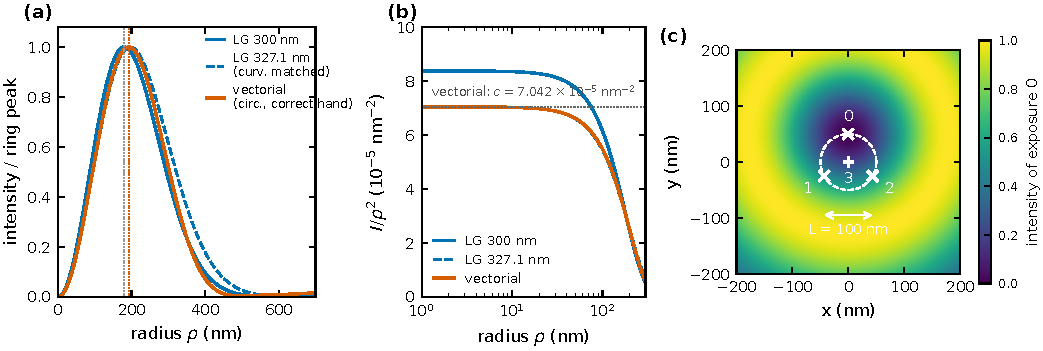
\includegraphics[width=\textwidth]{figures/fig1_schematic.pdf}
\caption{Beam model and TCP geometry. (a)~Normalized radial profiles of the scalar LG$_{01}$
donut ($\fwhm=\pnum{fwhm_nm}\src{fwhm_nm}$\,nm, Eq.~\ref{eq:lg}), of the LG donut with the zero
curvature of the vectorial donut ($\fwhm=\pnum{vectorial_lg_fwhm_curvature_nm}\src{vectorial_lg_fwhm_curvature_nm}$\,nm),
and of the vectorial Richards--Wolf vortex donut with circular polarization of the correct hand
($\lambda=640$\,nm, $\mathrm{NA}=1.4$, $n=1.518$, filling factor $5/3$); dotted lines mark the
ring radii, i.e.\ half the peak-to-peak diameters
\pnum{lg_ring_diameter_nm}\src{lg_ring_diameter_nm}\,nm (LG) and
\pnum{vectorial_peak_to_peak_diameter_nm}\src{vectorial_peak_to_peak_diameter_nm}\,nm
(vectorial). (b)~$I/\rho^2$ near the zero on a logarithmic radius axis: all zeros are quadratic,
the vectorial curvature is
$c=\pnum{vectorial_zero_curvature_nm2}\src{vectorial_zero_curvature_nm2}$\,nm$^{-2}$, and the
curvature-matched LG follows the vectorial profile for $\rho\lesssim100$\,nm. (c)~TCP: three
donut zeros ($\times$) on a circle of diameter $L$ (dashed; $L=100$\,nm shown for visibility)
plus a central exposure ($+$); the map is the intensity of exposure~0.}
\label{fig:schematic}
\end{figure*}

\section{Scalar versus vectorial donut (R1)}\label{sec:vectorial}

\emph{Zero and handedness.} With circular polarization of the correct hand every field component
of the focused vortex beam carries an azimuthal factor $e^{im\phi}$ with $m\neq0$, so the
on-axis intensity vanishes exactly at every $z$: the zero depth $I(0)/I_{\max}$ is
\pnum{vectorial_zero_depth_correct}\src{vectorial_zero_depth_correct} to machine precision. With
the opposite hand the longitudinal component $E_z$ does not vanish on axis and the zero fills to
\pnum{vectorial_zero_depth_wrong_handedness}\src{vectorial_zero_depth_wrong_handedness} of the
ring maximum; with linear polarization the depth is
\pnum{vectorial_zero_depth_linear}\src{vectorial_zero_depth_linear}
[Fig.~\ref{fig:vectorial}(a--d)], consistent with the experimental guidance on handedness of
Refs.~\cite{Lopez2023,Caprile2022}.

\emph{Equivalent LG donut.} The correct-hand vectorial ring has a peak-to-peak diameter
\pnum{vectorial_peak_to_peak_diameter_nm}\src{vectorial_peak_to_peak_diameter_nm}\,nm, and
near the zero $I/I_{\max}=c\rho^2$ with
$c=\pnum{vectorial_zero_curvature_nm2}\src{vectorial_zero_curvature_nm2}$\,nm$^{-2}$. The LG
donut of Eq.~\eqref{eq:lg} with the same curvature, $ea=c$, has
$\fwhm=\pnum{vectorial_lg_fwhm_curvature_nm}\src{vectorial_lg_fwhm_curvature_nm}$\,nm; the LG
donut with the same ring diameter would instead have
$\fwhm=\pnum{vectorial_lg_fwhm_diameter_nm}\src{vectorial_lg_fwhm_diameter_nm}$\,nm.

\emph{CRB.} Table~\ref{tab:vectorial} compares the centre CRB (limit $r\to0$ defined in
Sec.~\ref{sec:crb}, $N=100$, no background), with the vectorial beams evaluated exactly (no interpolation grid). The
curvature-matched LG donut reproduces the vectorial CRB to the ratios listed in the last rows
of the table, i.e.\ to a fraction of a percent up to $L=150$\,nm; the default LG donut with
$\fwhm=\pnum{fwhm_nm}\src{fwhm_nm}$\,nm overestimates it, with a ratio vectorial/LG of
\pnum{crb_vec_over_lg300_L150_N100}\src{crb_vec_over_lg300_L150_N100} at $L=150$\,nm and a
difference that keeps growing at larger $L$ [Fig.~\ref{fig:vectorial}(e,f)]. The overall
curvature of the beam cancels in the probabilities $p_i$: any exactly quadratic profile gives the
same CRB. The centre CRB is set by how the profile departs from quadratic at a distance $L/2$
from each zero [Eq.~\eqref{eq:master}, App.~\ref{app:derivation}]; with the peak normalized to
one, the curvature-matched LG donut happens to reproduce this departure for the vectorial beam
to a fraction of a percent. A filled zero, on the other hand, destroys the MINFLUX advantage, by
a factor that depends on $L$ (Table~\ref{tab:vectorial}): with the wrong hand the centre CRB
rises from \pnum{crb_center_vec_correct_L50_N100_nm}\src{crb_center_vec_correct_L50_N100_nm} to
\pnum{crb_center_vec_opposite_L50_N100_nm}\src{crb_center_vec_opposite_L50_N100_nm}\,nm at
$L=50$\,nm and from \pnum{crb_center_vec_correct_L150_N100_nm}\src{crb_center_vec_correct_L150_N100_nm}
to \pnum{crb_center_vec_opposite_L150_N100_nm}\src{crb_center_vec_opposite_L150_N100_nm}\,nm at
$L=150$\,nm, and with linear polarization to
\pnum{crb_center_vec_linear_L50_N100_nm}\src{crb_center_vec_linear_L50_N100_nm} and
\pnum{crb_center_vec_linear_L150_N100_nm}\src{crb_center_vec_linear_L150_N100_nm}\,nm,
respectively; the relative loss is largest at small $L$.

\begin{table}[b]
\caption{Centre CRB (nm; $r\to0$ limit, $N=100$, no background) of the TCP for the vectorial
donut (correct hand, opposite hand, linear polarization) and for LG donuts with the default
size parameter and with the curvature-matched one; last rows: CRB ratios.}
\label{tab:vectorial}
\begin{ruledtabular}
\begin{tabular}{lccc}
$L$ (nm) & $50$ & $100$ & $150$\\
\hline
vectorial, correct & \pnum{crb_center_vec_correct_L50_N100_nm}\src{crb_center_vec_correct_L50_N100_nm}
 & \pnum{crb_center_vec_correct_L100_N100_nm}\src{crb_center_vec_correct_L100_N100_nm}
 & \pnum{crb_center_vec_correct_L150_N100_nm}\src{crb_center_vec_correct_L150_N100_nm}\\
LG, curv.-matched & \pnum{crb_center_lgcurv_L50_N100_nm}\src{crb_center_lgcurv_L50_N100_nm}
 & \pnum{crb_center_lgcurv_L100_N100_nm}\src{crb_center_lgcurv_L100_N100_nm}
 & \pnum{crb_center_lgcurv_L150_N100_nm}\src{crb_center_lgcurv_L150_N100_nm}\\
LG, $\fwhm=\pnum{fwhm_nm}\src{fwhm_nm}$\,nm & \pnum{crb_center_lg300_L50_N100_nm}\src{crb_center_lg300_L50_N100_nm}
 & \pnum{crb_center_lg300_L100_N100_nm}\src{crb_center_lg300_L100_N100_nm}
 & \pnum{crb_center_lg300_L150_N100_nm}\src{crb_center_lg300_L150_N100_nm}\\
vectorial, opposite & \pnum{crb_center_vec_opposite_L50_N100_nm}\src{crb_center_vec_opposite_L50_N100_nm}
 & \pnum{crb_center_vec_opposite_L100_N100_nm}\src{crb_center_vec_opposite_L100_N100_nm}
 & \pnum{crb_center_vec_opposite_L150_N100_nm}\src{crb_center_vec_opposite_L150_N100_nm}\\
vectorial, linear & \pnum{crb_center_vec_linear_L50_N100_nm}\src{crb_center_vec_linear_L50_N100_nm}
 & \pnum{crb_center_vec_linear_L100_N100_nm}\src{crb_center_vec_linear_L100_N100_nm}
 & \pnum{crb_center_vec_linear_L150_N100_nm}\src{crb_center_vec_linear_L150_N100_nm}\\
\hline
ratio corr./curv. & \pnum{crb_vec_over_lgcurv_L50_N100}\src{crb_vec_over_lgcurv_L50_N100}
 & \pnum{crb_vec_over_lgcurv_L100_N100}\src{crb_vec_over_lgcurv_L100_N100}
 & \pnum{crb_vec_over_lgcurv_L150_N100}\src{crb_vec_over_lgcurv_L150_N100}\\
ratio corr./LG default & \pnum{crb_vec_over_lg300_L50_N100}\src{crb_vec_over_lg300_L50_N100}
 & \pnum{crb_vec_over_lg300_L100_N100}\src{crb_vec_over_lg300_L100_N100}
 & \pnum{crb_vec_over_lg300_L150_N100}\src{crb_vec_over_lg300_L150_N100}\\
\end{tabular}
\end{ruledtabular}
\end{table}

\begin{figure*}[t]
\centering
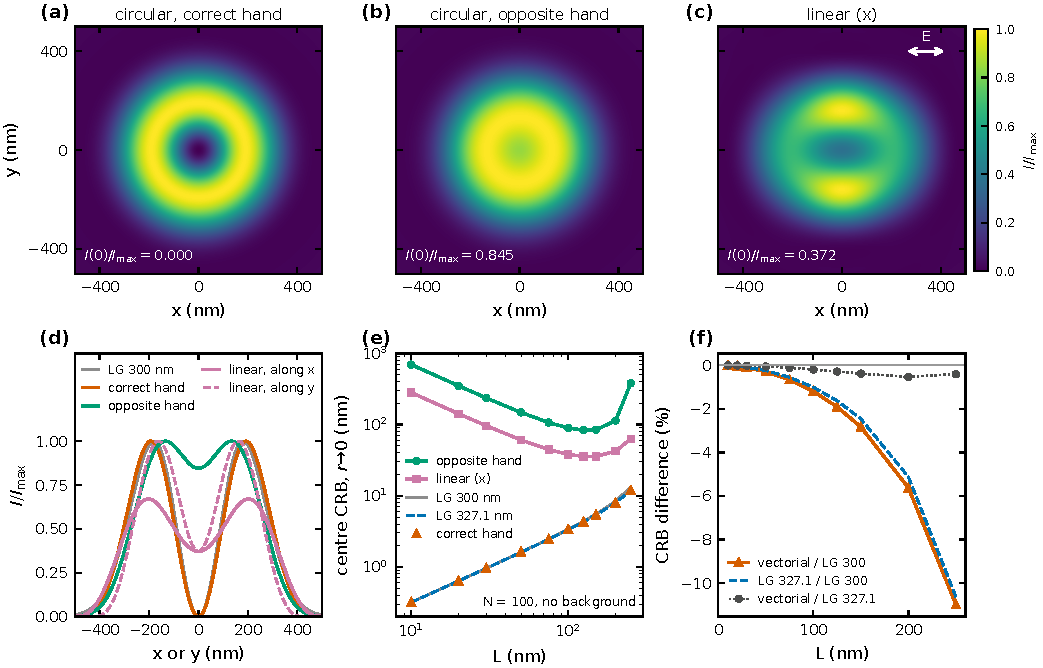
\includegraphics[width=\textwidth]{figures/fig2_vectorial.pdf}
\caption{Vectorial donut. (a--c)~Focal-plane intensity, normalized to the ring maximum, for
circular polarization of the correct hand, of the opposite hand, and for linear ($x$)
polarization. (d)~Profiles through the zero: the zero depth $I(0)/I_{\max}$ is
\pnum{vectorial_zero_depth_correct}\src{vectorial_zero_depth_correct} for the correct hand,
\pnum{vectorial_zero_depth_wrong_handedness}\src{vectorial_zero_depth_wrong_handedness} for the
opposite hand and \pnum{vectorial_zero_depth_linear}\src{vectorial_zero_depth_linear} for linear
polarization. (e)~Centre CRB ($r\to0$ limit, $N=100$, no background) of the TCP versus $L$; all
vectorial beams are evaluated exactly. (f)~Relative CRB differences: the vectorial donut and
the curvature-matched LG with respect to the LG donut with
$\fwhm=\pnum{fwhm_nm}\src{fwhm_nm}$\,nm, and (grey) the vectorial donut with respect to the
curvature-matched LG ($\fwhm=\pnum{vectorial_lg_fwhm_curvature_nm}\src{vectorial_lg_fwhm_curvature_nm}$\,nm),
not to the LG with $\fwhm=\pnum{fwhm_nm}\src{fwhm_nm}$\,nm; the latter CRB ratio is \pnum{crb_vec_over_lgcurv_L150_N100}\src{crb_vec_over_lgcurv_L150_N100} at
$L=150$\,nm.}
\label{fig:vectorial}
\end{figure*}

\section{The CRB at the TCP centre}\label{sec:crb}

\subsection{Point value and limit}
Write $x\equiv L^2\ln2/\fwhm^2$ and $g\equiv1-x$ ($x<1$, i.e.\ the peripheral zeros lie inside
the ring maximum). At $\rr=\mathbf0$ the central exposure has $p_3=0$ and $\nabla p_3=0$, so its
term in Eq.~\eqref{eq:fisher} is $0/0$. Dropping it gives the \emph{point value}, Balzarotti's
Eq.~S27 \cite{Balzarotti2017}:
\begin{equation}
\sigma_{\mathrm{pt}}=\frac{L}{2\sqrt{2N}}\,g^{-1}.
\label{eq:s27}
\end{equation}
For $\rr\neq\mathbf0$, however, $p_3\propto r^2$ and $\nabla p_3\propto\rr$, so the central term
tends to a finite matrix of fixed norm along $\rhat\rhat^{T}$. The limit $r\to0$ of the bound is
(App.~\ref{app:derivation})\src{deriv_limit}
\begin{equation}
\sigma_{\lim}^2=\frac{L^2}{8Ng^2}\,\frac{3g^2+e^{x}}{3g^2+2e^{x}},\qquad
\rho\equiv\frac{\sigma_{\lim}}{\sigma_{\mathrm{pt}}}=\sqrt{\frac{3g^2+e^{x}}{3g^2+2e^{x}}}.
\label{eq:limit}
\end{equation}
It does not depend on the direction of approach, so it is a well-defined, direction-independent
``centre CRB'' (the limiting error ellipse itself is anisotropic, see below). For $L=50$\,nm, $N=100$ and $\fwhm=\pnum{fwhm_nm}\src{fwhm_nm}$\,nm the numerical limit
of Eq.~\eqref{eq:crb} (12 directions at $|\rr|=10^{-3}$\,nm) is
\pnum{crb_center_lg_L50_N100_nm}\src{crb_center_lg_L50_N100_nm}\,nm and the closed form gives
\pnum{crb_center_lg_L50_N100_closed_nm}\src{crb_center_lg_L50_N100_closed_nm}\,nm, while the
point value is \pnum{crb_center_point_S27_L50_N100_nm}\src{crb_center_point_S27_L50_N100_nm}\,nm.
The closed forms agree with an independent numerical Fisher computation in all tested cases\src{check_closed_forms}. We use the limit because it describes an emitter at any small but
non-zero distance from the centre; the point value describes a set of measure zero.

For a quadratic zero ($x\to0$) the ratio is exactly $\rho=2/\sqrt5$, i.e.\
$\sigma^2_{\lim}=L^2/(10N)$ against $\sigma^2_{\mathrm{pt}}=L^2/(8N)$:
$\rho=\pnum{limit_to_point_ratio_quadratic}\src{limit_to_point_ratio_quadratic}$ (numerically,
with $\fwhm=10^9$\,nm, \pnum{limit_to_point_ratio_quadratic_numeric}\src{limit_to_point_ratio_quadratic_numeric}).
With finite $\fwhm$ the ratio is not conserved: at $\fwhm=\pnum{fwhm_nm}\src{fwhm_nm}$\,nm it is
\pnum{limit_to_point_ratio_L5}\src{limit_to_point_ratio_L5},
\pnum{limit_to_point_ratio_L50}\src{limit_to_point_ratio_L50},
\pnum{limit_to_point_ratio_L100}\src{limit_to_point_ratio_L100} and
\pnum{limit_to_point_ratio_L150}\src{limit_to_point_ratio_L150} for $L=5$, $50$, $100$ and
$150$\,nm [Fig.~\ref{fig:crbmaps}(f)], because the peripheral term scales as $g^2$ while the
central one scales as $e^{x}$.

\emph{Origin of the discontinuity.} The central term tends to $(\beta/N)\,\rhat\rhat^{T}$
($\alpha$ and $\beta$ are defined in Eq.~\eqref{eq:alphabeta}), which has a limit in norm but not as a matrix; equivalently $\sqrt{p_3}\propto|\rr|$ is a cone, so the
differentiability of $\sqrt{p}$ required by the Cram\'er--Rao theorem fails exactly at $r=0$\src{deriv_discontinuity}. The central exposure contributes only radial information, of the same
size at any distance (a quadratic zero is scale invariant), and a zero count is informative.
The limiting error ellipse is therefore anisotropic: $\sigma_\parallel=(\alpha+\beta)^{-1/2}$
along $\rhat$ and $\sigma_\perp=\sigma_{\mathrm{pt}}$ across it (App.~\ref{app:derivation}); for
$L=50$\,nm, $N=100$ these are
\pnum{crb_limit_axis_par_L50_N100_nm}\src{crb_limit_axis_par_L50_N100_nm}\,nm and
\pnum{crb_limit_axis_perp_L50_N100_nm}\src{crb_limit_axis_perp_L50_N100_nm}\,nm; for a quadratic
zero ($L=100$\,nm, $N=100$) \pnum{crb_limit_axis_par_L100_N100_quadratic_nm}\src{crb_limit_axis_par_L100_N100_quadratic_nm}\,nm
and \pnum{crb_limit_axis_perp_L100_N100_quadratic_nm}\src{crb_limit_axis_perp_L100_N100_quadratic_nm}\,nm,
with ratio $\sqrt{3/5}=\pnum{crb_limit_axis_ratio_quadratic}\src{crb_limit_axis_ratio_quadratic}$.

\subsection{Background: continuity and non-commuting limits}
With a finite SBR, $p_3\ge(1-s)/K>0$ with $s=\sbr/(\sbr+1)$, the central term vanishes as $r^2$
and the bound is continuous; the point value equals the limit and Balzarotti's Eq.~S31,
\begin{equation}
\crb(\mathbf0)=\frac{L}{2\sqrt{2N}}\,g^{-1}\sqrt{\Big(1+\frac{1}{\sbr}\Big)\Big(1+\frac{3}{4\,\sbr}\Big)}.
\label{eq:s31}
\end{equation}
For $\sbr=10$, $L=50$\,nm and $N=100$, Eq.~\eqref{eq:s31} gives
\pnum{crb_center_sbr10_L50_N100_nm}\src{crb_center_sbr10_L50_N100_nm}\,nm and the numerical
limit \pnum{crb_center_sbr10_limit_L50_N100_nm}\src{crb_center_sbr10_limit_L50_N100_nm}\,nm
[Fig.~\ref{fig:crbmaps}(e)]. The two limits do not commute\src{deriv_noncommuting}:
$\lim_{\sbr\to\infty}\lim_{r\to0}\crb=\sigma_{\mathrm{pt}}$ whereas
$\lim_{r\to0}\lim_{\sbr\to\infty}\crb=\sigma_{\lim}$; the central term switches on over a radius
$r_c\propto\sbr^{-1/2}$ that shrinks to a point [Fig.~\ref{fig:scaling}(c)]. To leading order
$r_c\simeq(\sqrt3L/4)\,e^{-x/2}/\sqrt{\sbr}$ (App.~\ref{app:derivation}): at realistic SBR it is
not small compared with $L$ (where the leading-order estimate is only indicative), and
Eq.~\eqref{eq:s31} is then the relevant centre value.

\subsection{Maps and scaling}
Figure~\ref{fig:crbmaps}(a--d) shows the CRB over the field of view for $L=50$ and $100$\,nm,
with and without background. The precision is best near the centre and degrades outside the
circle of zeros.

\emph{Scaling with $L$ and $N$.} For $L\ll\fwhm$ the centre CRB is linear in $L$: the log--log
slope over $L=5$--$40$\,nm is \pnum{crb_exponent_L}\src{crb_exponent_L}
[Fig.~\ref{fig:scaling}(a)]. The exponent is range dependent: over larger $L$ the factor
$g^{-1}$ steepens the curve, and with a perfect zero the bound diverges at the ring diameter
$L=\fwhm/\sqrt{\ln2}=\pnum{eps0_crb_divergence_L_nm}\src{eps0_crb_divergence_L_nm}$\,nm and
decreases beyond. The dependence on $N$ is exactly $N^{-1/2}$ (slope
$\pnum{crb_exponent_N}\src{crb_exponent_N}$ over $N=10^2$--$10^4$) for the limit, Eq.~\eqref{eq:s27} and Eq.~\eqref{eq:s31}
[Fig.~\ref{fig:scaling}(b)].

\emph{Photon cost of background.} The photons needed for a $5$\,nm centre CRB at $L=50$\,nm
(point value, Eqs.~\eqref{eq:s27} and~\eqref{eq:s31}) are
\pnum{photons_for_5nm_L50_sbrinf}\src{photons_for_5nm_L50_sbrinf},
\pnum{photons_for_5nm_L50_sbr50}\src{photons_for_5nm_L50_sbr50},
\pnum{photons_for_5nm_L50_sbr20}\src{photons_for_5nm_L50_sbr20},
\pnum{photons_for_5nm_L50_sbr10}\src{photons_for_5nm_L50_sbr10} and
\pnum{photons_for_5nm_L50_sbr5}\src{photons_for_5nm_L50_sbr5} for $\sbr=\infty$, $50$, $20$,
$10$ and $5$; with the background-free limit it would be
\pnum{photons_for_5nm_L50_limit_nobg}\src{photons_for_5nm_L50_limit_nobg}.

\emph{Comparison with published values and variants.} With $N=500$ and $\sbr=5$,
Eq.~\eqref{eq:s31} gives \pnum{crb_center_sbr5_N500_fwhm360_L50_nm}\src{crb_center_sbr5_N500_fwhm360_L50_nm},
\pnum{crb_center_sbr5_N500_fwhm360_L100_nm}\src{crb_center_sbr5_N500_fwhm360_L100_nm} and
\pnum{crb_center_sbr5_N500_fwhm360_L150_nm}\src{crb_center_sbr5_N500_fwhm360_L150_nm}\,nm for
$L=50$, $100$, $150$\,nm when $\fwhm=\pnum{fwhm_masullo_nm}\src{fwhm_masullo_nm}$\,nm. These
match, up to rounding in the last digit at $L=150$\,nm, the MINFLUX centre-precision column of
Supplementary Table~1 of Masullo \textit{et al.} \cite{Masullo2022}\src{lit_masullo_table};
that table legend states no SBR or $N$ for this column, so $\sbr=5$, $N=500$ and this $\fwhm$
are our inference from the other columns. By contrast, with $\fwhm=\pnum{fwhm_nm}\src{fwhm_nm}$\,nm the same
formula gives \pnum{crb_center_sbr5_N500_fwhm300_L50_nm}\src{crb_center_sbr5_N500_fwhm300_L50_nm},
\pnum{crb_center_sbr5_N500_fwhm300_L100_nm}\src{crb_center_sbr5_N500_fwhm300_L100_nm} and
\pnum{crb_center_sbr5_N500_fwhm300_L150_nm}\src{crb_center_sbr5_N500_fwhm300_L150_nm}\,nm. The
one-dimensional two-exposure bound $L/(4\sqrt N)$ (Balzarotti Eq.~S22c) is
\pnum{crb_1d_quadratic_L50_N100_nm}\src{crb_1d_quadratic_L50_N100_nm}\,nm for $L=50$\,nm,
$N=100$. With a multiphoton exponent $c$ ($\lambda_i\propto I_i^c$
\cite{MasulloStefani2022}) the point value is $\sigma_{\mathrm{pt}}/c$\src{deriv_multiphoton}: \pnum{crb_center_multiphoton_c1_L100_N100_quadratic_nm}\src{crb_center_multiphoton_c1_L100_N100_quadratic_nm},
\pnum{crb_center_multiphoton_c2_L100_N100_quadratic_nm}\src{crb_center_multiphoton_c2_L100_N100_quadratic_nm}
and \pnum{crb_center_multiphoton_c3_L100_N100_quadratic_nm}\src{crb_center_multiphoton_c3_L100_N100_quadratic_nm}\,nm
for $c=1$, $2$, $3$ ($L=100$\,nm, $N=100$, quadratic zero); for $c>1$ the central term vanishes
at the origin and there is no discontinuity.

\begin{figure*}[t]
\centering
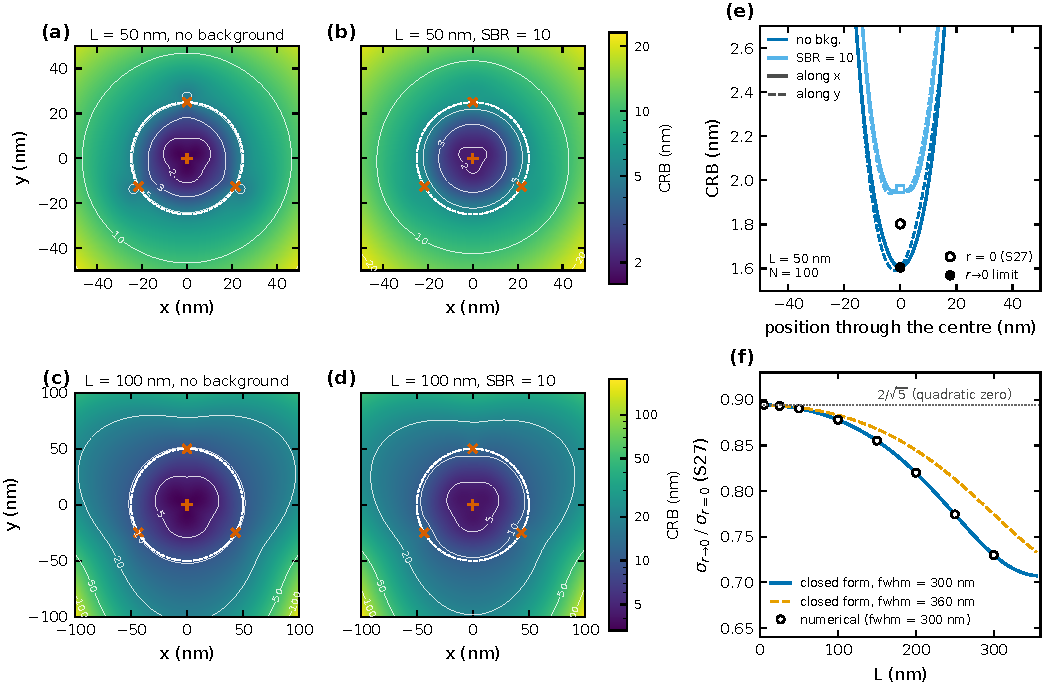
\includegraphics[width=\textwidth]{figures/fig3_crb_maps.pdf}
\caption{CRB maps and the discontinuity at the TCP centre ($\fwhm=\pnum{fwhm_nm}\src{fwhm_nm}$\,nm,
$N=100$). (a--d)~CRB over the field of view $|x|,|y|\le L$ for $L=50$ and $100$\,nm, without
background and with $\sbr=10$ (logarithmic colour scale, contours in nm; pixels on a perfect
zero take the $r\to0$ limit). (e)~Cuts through the centre along $x$ and $y$ for $L=50$\,nm:
without background the $r\to0$ limit
(\pnum{crb_center_lg_L50_N100_nm}\src{crb_center_lg_L50_N100_nm}\,nm, filled circle) lies below
the point value of Eq.~\eqref{eq:s27}
(\pnum{crb_center_point_S27_L50_N100_nm}\src{crb_center_point_S27_L50_N100_nm}\,nm, open
circle), which excludes the central exposure with $p=0$; with $\sbr=10$ the CRB is continuous
(Eq.~\eqref{eq:s31}, \pnum{crb_center_sbr10_L50_N100_nm}\src{crb_center_sbr10_L50_N100_nm}\,nm).
(f)~Ratio of the limit to the point value versus $L$, closed form (lines) and numerical Fisher
computation (circles), with the closed form for
$\fwhm=\pnum{fwhm_masullo_nm}\src{fwhm_masullo_nm}$\,nm dashed; it tends to $2/\sqrt5$ only for a quadratic zero ($L\ll\fwhm$).}
\label{fig:crbmaps}
\end{figure*}

\begin{figure*}[t]
\centering
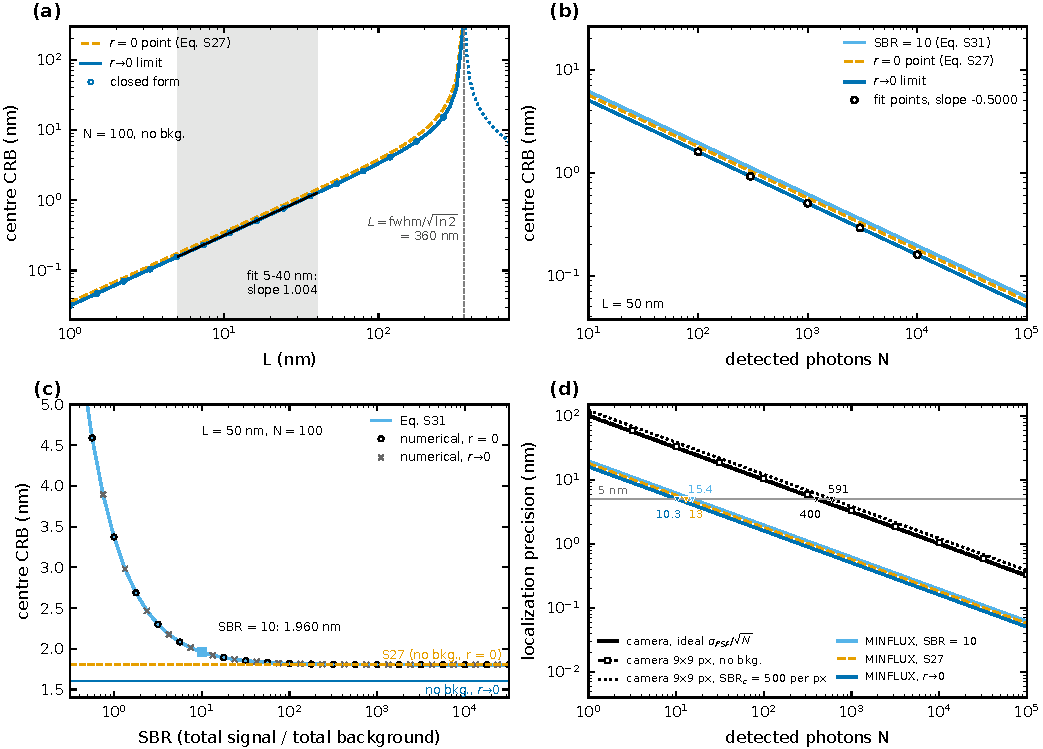
\includegraphics[width=\textwidth]{figures/fig4_scaling.pdf}
\caption{Scaling of the centre CRB and comparison with camera localization. (a)~CRB versus $L$
($N=100$, no background): $r\to0$ limit (numerical and closed form) and point value of
Eq.~\eqref{eq:s27}; the log--log slope fitted over $L=5$--$40$\,nm (shaded, $L\ll\fwhm$) is
\pnum{crb_exponent_L}\src{crb_exponent_L}. With a perfect zero the CRB increases monotonically
only for $L$ below the ring diameter
\pnum{eps0_crb_divergence_L_nm}\src{eps0_crb_divergence_L_nm}\,nm, diverges there and decreases
beyond (dotted). (b)~CRB versus $N$ for $L=50$\,nm: slope $-1/2$ for the limit, the point value
and Eq.~\eqref{eq:s31} with $\sbr=10$. (c)~CRB versus SBR ($L=50$\,nm, $N=100$): for finite SBR
the point value equals the limit (Eq.~\eqref{eq:s31}) and, as $\sbr\to\infty$, tends to the
point value of Eq.~\eqref{eq:s27}, not to the background-free limit. (d)~MINFLUX ($L=50$\,nm)
versus a camera ($\sigma_{\mathrm{PSF}}=100$\,nm): continuum limit $\sigma_{\mathrm{PSF}}/\sqrt N$
and a $9\times9$ window of $100$\,nm pixels, without background (dashed, nearly coincident with
the continuum line) and with $\sbr_c=500$ defined per pixel (total SBR \pnum{camera_sbr_perpixel_to_total}\src{camera_sbr_perpixel_to_total});
triangles mark the photons needed for $5$\,nm: $400$ for the ideal camera
(\pnum{camera_ideal_N400_nm}\src{camera_ideal_N400_nm}\,nm at $N=400$),
\pnum{camera_photons_for_5nm_perpixel_sbr500}\src{camera_photons_for_5nm_perpixel_sbr500} for
the pixelated camera with background, and for MINFLUX
\pnum{photons_for_5nm_L50_limit_nobg}\src{photons_for_5nm_L50_limit_nobg} with the $r\to0$
limit, \pnum{photons_for_5nm_L50_sbrinf}\src{photons_for_5nm_L50_sbrinf} with the point value
and \pnum{photons_for_5nm_L50_sbr10}\src{photons_for_5nm_L50_sbr10} with $\sbr=10$.}
\label{fig:scaling}
\end{figure*}

\section{Estimators versus the CRB (R3)}\label{sec:estimators}

All MC results in this section use $L=50$\,nm, $\fwhm=\pnum{fwhm_nm}\src{fwhm_nm}$\,nm, seed
$42$ and $10^4$ repetitions unless stated otherwise; standard errors (SE) of $\sigma$ are
nonparametric bootstrap estimates.

\emph{MLE with background: efficient at the centre.} With $\sbr=10$ the model is regular at the
centre ($p_3>0$). For $N=100$ and an MLE search disk of radius $L$, the MLE precision is
$\sigma=\pnum{mle_sigma_center_sbr10_nm}\pm\pnumse{mle_sigma_center_sbr10_nm}$\src{mle_sigma_center_sbr10_nm}\,nm
against the bound \pnum{crb_center_sbr10_L50_N100_nm}\src{crb_center_sbr10_L50_N100_nm}\,nm of
Eq.~\eqref{eq:s31}: an efficiency
$\sigma/\crb=\pnum{mle_efficiency_center}\pm\pnumse{mle_efficiency_center}$\src{mle_efficiency_center}.
This is the value we define as the MLE efficiency at the centre; the choice $\sbr=10$ (a
regular, physical case) is a declared convention (Sec.~\ref{sec:open}).

\emph{MLE without background: biased and superefficient.} Without background $p_3\propto r^2$,
the model is not regular at the centre, and the MLE beats the CRB limit:
$\sigma=\pnum{mle_nobg_sigma_center_nm}\pm\pnumse{mle_nobg_sigma_center_nm}$\src{mle_nobg_sigma_center_nm}\,nm,
i.e.\ $\sigma/\sigma_{\lim}=\pnum{mle_nobg_sigma_over_crb_limit_center}\pm\pnumse{mle_nobg_sigma_over_crb_limit_center}$\src{mle_nobg_sigma_over_crb_limit_center}
and $\sigma/\sigma_{\mathrm{pt}}=\pnum{mle_nobg_sigma_over_s27_center}\pm\pnumse{mle_nobg_sigma_over_s27_center}$\src{mle_nobg_sigma_over_s27_center}
at $N=100$. The ratio does not approach one as $N$ grows [Fig.~\ref{fig:estimators}(c)], so this
is not a small-$N$ effect. The price is a bias, toward the centre close to it
[for $x_0\lesssim8$\,nm, Fig.~\ref{fig:estimators}(d)]: at $\rr=(2,0)$\,nm the mean
error along $x$ is
$\pnum{mle_nobg_bias_x_r2_nm}\pm\pnumse{mle_nobg_bias_x_r2_nm}$\src{mle_nobg_bias_x_r2_nm}\,nm
($4\times10^4$ repetitions) [Fig.~\ref{fig:estimators}(d)]. The CRB bounds only unbiased
estimators of a regular model, so there is no contradiction; it means that, without background,
neither the point value nor the limit is a bound on what an MLE reports near the centre.

\emph{LMS.} Without background the LMS estimate at the centre has exactly the covariance of the
point value, $L^2/(8Ng^2)$ per axis\src{lms_center_analytic}: in MC,
$\sigma/\sigma_{\mathrm{pt}}=\pnum{lms_nobg_sigma_over_s27_center}\pm\pnumse{lms_nobg_sigma_over_s27_center}$\src{lms_nobg_sigma_over_s27_center}
and $\sigma/\sigma_{\lim}=\pnum{lms_nobg_sigma_over_crb_limit_center}\pm\pnumse{lms_nobg_sigma_over_crb_limit_center}$\src{lms_nobg_sigma_over_crb_limit_center}
($=1/\rho$), constant in $N$ [Fig.~\ref{fig:estimators}(c)]. With background, the expectation of the LMS of
Balzarotti Eq.~S50 without the $1/s$ correction is exactly $s=\sbr/(\sbr+1)$ times that of the
background-free LMS at every position\src{lms_sbr_shrink} (the constant background term cancels
because $\sum_k\bb_k=\mathbf0$). In Fig.~\ref{fig:estimators}(a,b) the LMS and mLMS include the
$1/s$ correction. Beyond $x_0\approx15$\,nm they are strongly biased toward the centre
[Fig.~\ref{fig:estimators}(a)], because the linearization compresses the estimate, and their
$\sigma$ falls below the CRB [Fig.~\ref{fig:estimators}(b)]; this reflects the compression, not a
gain in precision. Closer to the centre this does not hold: for $x_0\lesssim12$\,nm the mLMS has
$\sigma$ above the CRB, and for $x_0\approx5$--$15$\,nm its bias is small and slightly outward.

\emph{MLE away from the centre: an outlier tail at low $N$.} With $\sbr=10$ and $N=100$ the MLE
is not efficient everywhere inside the TCP. At $\rr=(15,0)$\,nm, with a search disk of radius
$2L$, $\sigma/\crb=\pnum{mle_sbr10_sigma_over_crb_x15_N100}\pm\pnumse{mle_sbr10_sigma_over_crb_x15_N100}$\src{mle_sbr10_sigma_over_crb_x15_N100},
caused by a tail of outliers (the bump in Fig.~\ref{fig:estimators}(b) for $x_0\approx10$--$20$\,nm);
at $N=1000$ it is
$\pnum{mle_sbr10_sigma_over_crb_x15_N1000}\pm\pnumse{mle_sbr10_sigma_over_crb_x15_N1000}$\src{mle_sbr10_sigma_over_crb_x15_N1000}.
The size of the tail depends on the search radius, which must therefore be reported with any
such number; the convergence of the MLE to the CRB away from the centre only at larger $N$ agrees
with Ref.~\cite{Balzarotti2017}.

\begin{figure*}[t]
\centering
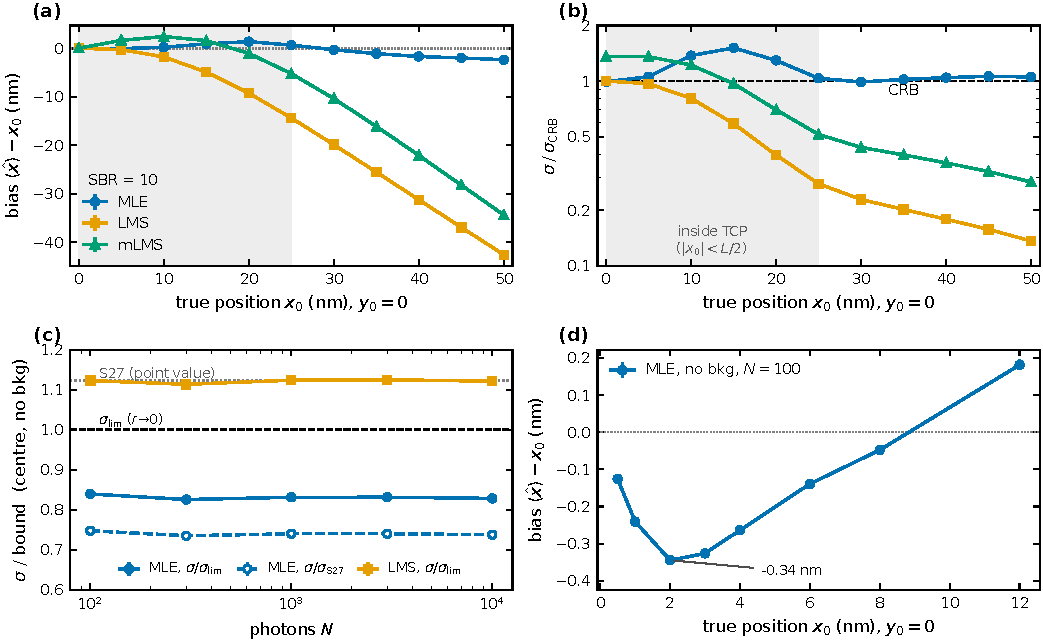
\includegraphics[width=\textwidth]{figures/fig5_estimators.pdf}
\caption{Estimators versus the CRB ($L=50$\,nm, $N=100$ unless indicated, seed 42).
(a)~Bias and (b)~$\sigma/\crb$ versus the emitter position $x_0$ along $x$, from the centre to
$L$ (inside the TCP shaded), for the MLE, the LMS and the mLMS with $\sbr=10$; off-centre MLE
points use a search disk of radius $2L$, and the centre point (radius $L$, $10^4$ repetitions)
equals the efficiency
$\pnum{mle_efficiency_center}\src{mle_efficiency_center}$. The MLE bump in (b) at
$x_0\approx10$--$20$\,nm ($\sigma/\crb=\pnum{mle_sbr10_sigma_over_crb_x15_N100}\src{mle_sbr10_sigma_over_crb_x15_N100}$
at $x_0=15$\,nm) is an outlier tail whose size depends on the $2L$ search radius. (c)~Centre,
no background: $\sigma$ of the MLE divided by the $r\to0$ limit (superefficiency,
\pnum{mle_nobg_sigma_over_crb_limit_center}\src{mle_nobg_sigma_over_crb_limit_center} at
$N=100$) and by the point value of Eq.~\eqref{eq:s27}
(\pnum{mle_nobg_sigma_over_s27_center}\src{mle_nobg_sigma_over_s27_center}), and $\sigma$ of the
LMS divided by the limit, versus $N$. (d)~Bias of the background-free MLE near the centre
versus $x_0$ ($N=100$): negative (toward the centre) for $x_0\lesssim8$\,nm, with
$\pnum{mle_nobg_bias_x_r2_nm}\pm\pnumse{mle_nobg_bias_x_r2_nm}$\src{mle_nobg_bias_x_r2_nm}\,nm
at $\rr=(2,0)$\,nm, and changing sign (away from the centre) near $x_0\approx9$\,nm.}
\label{fig:estimators}
\end{figure*}

\section{Camera reference (R2)}\label{sec:camera}

As a reference we use the CRB of a camera with a Gaussian point-spread function of
$\sigma_{\mathrm{PSF}}=100$\,nm \cite{Balzarotti2017}. In the continuum limit without background
the bound is $\sigma_{\mathrm{PSF}}/\sqrt N$:
\pnum{camera_ideal_N400_nm}\src{camera_ideal_N400_nm}\,nm for $N=400$ and
\pnum{camera_sigma_nm}\src{camera_sigma_nm}\,nm for $N=1000$; this \emph{ideal} value is the
camera reference of Sec.~\ref{sec:iterative}. Pixelation costs little: a $9\times9$ window of
$100$\,nm pixels gives \pnum{camera_pixelated_9x9_N400_nm}\src{camera_pixelated_9x9_N400_nm}\,nm
at $N=400$ and \pnum{camera_pixelated_9x9_N1000_nm}\src{camera_pixelated_9x9_N1000_nm}\,nm at
$N=1000$.

The SBR convention matters for the camera. Balzarotti's $\sbr_c$ is the total signal over the
background \emph{per pixel} (Eq.~S61), so $\sbr_c=500$ on $9\times9$ pixels corresponds to a total
SBR of \pnum{camera_sbr_perpixel_to_total}\src{camera_sbr_perpixel_to_total}. With that
convention the pixelated camera reaches
\pnum{camera_perpixel_sbr500_N600_nm}\src{camera_perpixel_sbr500_N600_nm}\,nm at $N=600$ and
needs \pnum{camera_photons_for_5nm_perpixel_sbr500}\src{camera_photons_for_5nm_perpixel_sbr500}
photons for $5$\,nm; if $500$ were the total SBR it would reach
\pnum{camera_total_sbr500_N600_nm}\src{camera_total_sbr500_N600_nm}\,nm and need
\pnum{camera_photons_for_5nm_total_sbr500}\src{camera_photons_for_5nm_total_sbr500} photons. The
SBR values of MINFLUX (total/total) and of the camera (total/per pixel) are therefore not
directly comparable. For comparison, MINFLUX with $L=50$\,nm and $\sbr=10$ needs
\pnum{photons_for_5nm_L50_sbr10}\src{photons_for_5nm_L50_sbr10} photons for a $5$\,nm centre CRB
[Fig.~\ref{fig:scaling}(d)].

\section{Iterative MINFLUX (R4)}\label{sec:iterative}

\emph{Protocol.} The emitter is placed uniformly in a disk of radius $L_0/4$ around the initial
pattern centre. Four iterations use TCPs of geometrically decreasing diameter
$L_k=150\to25$\,nm with an equal share of the total photon budget $N_{\mathrm{tot}}$; each
pattern is re-centred on the previous estimate, and each estimate is an MLE in a disk of radius
$0.75L_k$ around the current centre. Unless stated otherwise there is no background, and each
point uses $10^4$ repetitions (seed 42) with bootstrap SE. The iterative scheme was proposed
qualitatively in Ref.~\cite{Balzarotti2017} and relies on the scale invariance of a quadratic
zero \cite{Stefani2023}.

\emph{Precision and camera comparison.} For $N_{\mathrm{tot}}=1000$ the final precision is
$\sigma=\pnum{iterative_sigma_nm}\pm\pnumse{iterative_sigma_nm}$\src{iterative_sigma_nm}\,nm,
i.e.\ \pnum{iterative_ratio_to_camera_N1000}\,$\pm$\,\pnumse{iterative_ratio_to_camera_N1000}\src{iterative_ratio_to_camera_N1000}
times the ideal camera value \pnum{camera_sigma_nm}\src{camera_sigma_nm}\,nm with the same
photons; with $\sbr=10$ it is
\pnum{iterative_sbr10_sigma_nm}\,$\pm$\,\pnumse{iterative_sbr10_sigma_nm}\src{iterative_sbr10_sigma_nm}\,nm.
For reference, spending all photons at the final $L=25$\,nm with the emitter at the centre
would give \pnum{iterative_crb_all_photons_L25_N1000_nm}\src{iterative_crb_all_photons_L25_N1000_nm}\,nm;
the iterations pay for their field of view with photons spent at large $L$
[Fig.~\ref{fig:iterative}(a,c)].

\emph{Photon scaling.} Over $N_{\mathrm{tot}}=250$, $500$, $1000$, $2000$, $4000$, $8000$ the
final precision is \pnum{iterative_sigma_N250_nm}\src{iterative_sigma_N250_nm},
\pnum{iterative_sigma_N500_nm}\src{iterative_sigma_N500_nm},
\pnum{iterative_sigma_N1000_nm}\src{iterative_sigma_N1000_nm},
\pnum{iterative_sigma_N2000_nm}\src{iterative_sigma_N2000_nm},
\pnum{iterative_sigma_N4000_nm}\src{iterative_sigma_N4000_nm} and
\pnum{iterative_sigma_N8000_nm}\src{iterative_sigma_N8000_nm}\,nm. The log--log slope for
$N_{\mathrm{tot}}\ge500$ is
$\pnum{iterative_slope_N_ge_500}\pm\pnumse{iterative_slope_N_ge_500}$\src{iterative_slope_N_ge_500}
(bootstrap 95\% interval $[\pnum{iterative_slope_N_ge_500_ci95_lo}\src{iterative_slope_N_ge_500_ci95_lo},
\pnum{iterative_slope_N_ge_500_ci95_hi}\src{iterative_slope_N_ge_500_ci95_hi}]$), which excludes
$-1/2$: the iterative scheme improves slightly faster than $N^{-1/2}$ (we have not isolated the
mechanism; a plausible one is the better centring of the later iterations). Over the full range
the slope is $\pnum{iterative_slope_all}\src{iterative_slope_all}$
($[\pnum{iterative_slope_all_ci95_lo}\src{iterative_slope_all_ci95_lo},
\pnum{iterative_slope_all_ci95_hi}\src{iterative_slope_all_ci95_hi}]$), but it is driven by a
heavy-tailed error distribution at $N_{\mathrm{tot}}=250$, where the bootstrap SE
(\pnumse{iterative_sigma_N250_nm}\,nm) is itself unstable. The ratio to the ideal camera falls
from \pnum{iterative_ratio_max}\src{iterative_ratio_max} at $N_{\mathrm{tot}}=250$ to
\pnum{iterative_ratio_min}\src{iterative_ratio_min} and flattens [Fig.~\ref{fig:iterative}(b)].

\emph{Adaptive schedule.} A rule $L_{k+1}=\max(L_{\min},\kappa\sigma_k)$ with $\kappa=6$ and
$\sigma_k$ the centre CRB of iteration $k$ gives $L=150,25,25,25$\,nm and
$\sigma=\pnum{iterative_adaptive_sigma_nm}\pm\pnumse{iterative_adaptive_sigma_nm}$\src{iterative_adaptive_sigma_nm}\,nm
at $N_{\mathrm{tot}}=1000$. The rule is less safe than it looks: the centre CRB of iteration~0
(\pnum{adaptive_iter0_crb_center_nm}\src{adaptive_iter0_crb_center_nm}\,nm) underestimates the
real error (\pnum{adaptive_iter0_sigma_nm}\,$\pm$\,\pnumse{adaptive_iter0_sigma_nm}\src{adaptive_iter0_sigma_nm}\,nm),
because the emitter is not at the centre of the first pattern, and a fraction
\pnum{adaptive_frac_outside_next_radius}\,$\pm$\,\pnumse{adaptive_frac_outside_next_radius}\src{adaptive_frac_outside_next_radius}
of the emitters ends up outside the radius $L_1/2$ of the next pattern.

\emph{Without re-centring.} If the patterns are not re-centred the final $\sigma$ is
\pnum{iterative_no_recenter_sigma_nm_ARTEFACT}\src{iterative_no_recenter_sigma_nm_ARTEFACT}\,nm
and worsens in the last iteration. This is an artefact of the protocol, not physics: the MLE
search disk ($0.75L_k$) becomes smaller than the spread of emitter positions ($L_0/4$), and the
estimates are truncated. The point is shown in grey in Fig.~\ref{fig:iterative}(a) and not used
elsewhere.

\begin{figure*}[t]
\centering
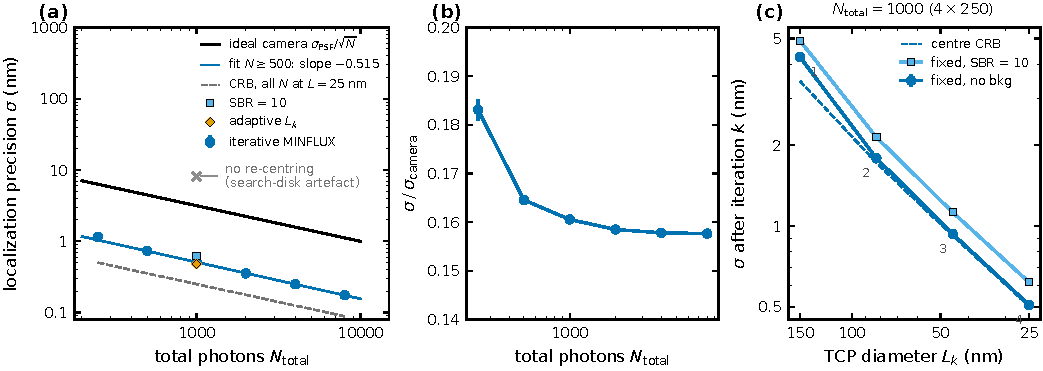
\includegraphics[width=\textwidth]{figures/fig6_iterative.pdf}
\caption{Iterative MINFLUX versus camera localization (4 iterations, $L_k=150\to25$\,nm, equal
photon split, re-centring, MLE, no background, $10^4$ repetitions). (a)~Final precision
($\sigma\pm$ bootstrap SE) versus total photon budget, with the ideal camera
$\sigma_{\mathrm{PSF}}/\sqrt N$, the fitted slope for $N_{\mathrm{tot}}\ge500$
($\pnum{iterative_slope_N_ge_500}\src{iterative_slope_N_ge_500}$), the centre CRB if all photons
were spent at $L=25$\,nm, and single points with $\sbr=10$ and with the adaptive schedule at
$N_{\mathrm{tot}}=1000$; the grey cross (no re-centring) is an artefact of the truncated search
disk. (b)~$\sigma/\sigma_{\mathrm{camera}}$ versus $N_{\mathrm{tot}}$, from
\pnum{iterative_ratio_max}\src{iterative_ratio_max} to
\pnum{iterative_ratio_min}\src{iterative_ratio_min}. (c)~$\sigma$ after each iteration versus the
pattern diameter $L_k$ for $N_{\mathrm{tot}}=1000$, without background and with $\sbr=10$,
compared with the centre CRB of each iteration.}
\label{fig:iterative}
\end{figure*}

\section{Non-idealities (R5)}\label{sec:nonideal}

\subsection{Finite zero depth}
Experimental donuts have a residual intensity $\epsilon$ at the zero, relative to the ring
maximum (below $0.2\%$ in Ref.~\cite{Balzarotti2017}\src{lit_balzarotti_zero_depth}). We model it
in two ways (App.~\ref{app:derivation}): a \emph{constant} pedestal, $I=I_{\mathrm{LG}}+\epsilon$,
and a \emph{Gaussian} pedestal, $I=(ea\rho^2+\epsilon)e^{-a\rho^2}$. The constant pedestal is
exactly a background: at the centre the CRB is Eq.~\eqref{eq:s31} with
$\sbr_\epsilon=3e\,x\,e^{-x}/(4\epsilon)$; the Gaussian pedestal is not equivalent to any
background, because it differs between exposures and reduces the slope of the donut\src{deriv_pedestal}. With $\epsilon>0$ the point value equals the limit and tends, as
$\epsilon\to0$, to the point value $\sigma_{\mathrm{pt}}$, not to $\sigma_{\lim}$.

\emph{Degradation at fixed $L$.} Table~\ref{tab:eps} lists
$\crb(\epsilon)/\sigma_{\mathrm{pt}}$ at the centre. The loss is largest for small $L$, since
$\sbr_\epsilon\propto x\propto L^2$: at $L=50$\,nm a pedestal of $5\%$ roughly doubles the CRB.
The two pedestal models agree to first order in $\epsilon$ up to corrections of relative order
$x^2$\src{deriv_pedestal}.

\begin{table}[b]
\caption{Centre CRB with a finite zero depth $\epsilon$, relative to the point value of
Eq.~\eqref{eq:s27} ($\fwhm=\pnum{fwhm_nm}\src{fwhm_nm}$\,nm, no background); constant /
Gaussian pedestal.}
\label{tab:eps}
\begin{ruledtabular}
\begin{tabular}{lcc}
$\epsilon$ & $L=50$\,nm & $L=100$\,nm\\
\hline
0.002 & \pnum{crb_eps_degradation_L50_eps0p002_constant}\src{crb_eps_degradation_L50_eps0p002_constant} / \pnum{crb_eps_degradation_L50_eps0p002_gaussian}\src{crb_eps_degradation_L50_eps0p002_gaussian}
 & \pnum{crb_eps_degradation_L100_eps0p002_constant}\src{crb_eps_degradation_L100_eps0p002_constant} / \pnum{crb_eps_degradation_L100_eps0p002_gaussian}\src{crb_eps_degradation_L100_eps0p002_gaussian}\\
0.01 & \pnum{crb_eps_degradation_L50_eps0p01_constant}\src{crb_eps_degradation_L50_eps0p01_constant} / \pnum{crb_eps_degradation_L50_eps0p01_gaussian}\src{crb_eps_degradation_L50_eps0p01_gaussian}
 & \pnum{crb_eps_degradation_L100_eps0p01_constant}\src{crb_eps_degradation_L100_eps0p01_constant} / \pnum{crb_eps_degradation_L100_eps0p01_gaussian}\src{crb_eps_degradation_L100_eps0p01_gaussian}\\
0.05 & \pnum{crb_eps_degradation_L50_eps0p05_constant}\src{crb_eps_degradation_L50_eps0p05_constant} / \pnum{crb_eps_degradation_L50_eps0p05_gaussian}\src{crb_eps_degradation_L50_eps0p05_gaussian}
 & \pnum{crb_eps_degradation_L100_eps0p05_constant}\src{crb_eps_degradation_L100_eps0p05_constant} / \pnum{crb_eps_degradation_L100_eps0p05_gaussian}\src{crb_eps_degradation_L100_eps0p05_gaussian}\\
0.15 & \pnum{crb_eps_degradation_L50_eps0p15_constant}\src{crb_eps_degradation_L50_eps0p15_constant} / \pnum{crb_eps_degradation_L50_eps0p15_gaussian}\src{crb_eps_degradation_L50_eps0p15_gaussian}
 & \pnum{crb_eps_degradation_L100_eps0p15_constant}\src{crb_eps_degradation_L100_eps0p15_constant} / \pnum{crb_eps_degradation_L100_eps0p15_gaussian}\src{crb_eps_degradation_L100_eps0p15_gaussian}\\
\end{tabular}
\end{ruledtabular}
\end{table}

\emph{Optimal $L$.} Because shrinking $L$ makes the pedestal relatively larger, the centre CRB
(Gaussian pedestal, $N=100$) has a minimum at an optimal diameter [Fig.~\ref{fig:zerodepth}(a)]:
$L_{\mathrm{opt}}=\pnum{L_opt_eps0p002_nm}\src{L_opt_eps0p002_nm}$,
\pnum{L_opt_eps0p01_nm}\src{L_opt_eps0p01_nm}, \pnum{L_opt_eps0p05_nm}\src{L_opt_eps0p05_nm} and
\pnum{L_opt_eps0p15_nm}\src{L_opt_eps0p15_nm}\,nm, with a CRB of
\pnum{crb_opt_eps0p002_nm}\src{crb_opt_eps0p002_nm},
\pnum{crb_opt_eps0p01_nm}\src{crb_opt_eps0p01_nm}, \pnum{crb_opt_eps0p05_nm}\src{crb_opt_eps0p05_nm}
and \pnum{crb_opt_eps0p15_nm}\src{crb_opt_eps0p15_nm}\,nm, for $\epsilon=0.002$, $0.01$, $0.05$ and
$0.15$. In units of $\fwhm\sqrt\epsilon$ the optimum is
\pnum{L_opt_over_fwhm_sqrt_eps_eps0p002}\src{L_opt_over_fwhm_sqrt_eps_eps0p002},
\pnum{L_opt_over_fwhm_sqrt_eps_eps0p01}\src{L_opt_over_fwhm_sqrt_eps_eps0p01},
\pnum{L_opt_over_fwhm_sqrt_eps_eps0p05}\src{L_opt_over_fwhm_sqrt_eps_eps0p05} and
\pnum{L_opt_over_fwhm_sqrt_eps_eps0p15}\src{L_opt_over_fwhm_sqrt_eps_eps0p15}, independent of
$\fwhm$: the rule $L_{\mathrm{opt}}\approx\pnum{L_opt_over_fwhm_sqrt_eps_eps0p002}\src{L_opt_over_fwhm_sqrt_eps_eps0p002}\,\fwhm\sqrt\epsilon$
holds only for $\epsilon\lesssim0.01$ [Fig.~\ref{fig:zerodepth}(b)]. With $\epsilon=0$ there is no
optimum; the CRB grows monotonically up to the divergence at the ring diameter,
\pnum{eps0_crb_divergence_L_nm}\src{eps0_crb_divergence_L_nm}\,nm.

\emph{Off-centre minimum.} With a nearly perfect zero the CRB minimum moves off the centre
[Fig.~\ref{fig:zerodepth}(c), $\epsilon=0.002$, $L=100$\,nm]: the pedestal dominates the zero
within a radius of order $\sqrt{\epsilon/(ea)}=\pnum{zero_depth_transition_scale_nm}\src{zero_depth_transition_scale_nm}$\,nm,
independent of $L$. This is a scale, not the position of the minimum, which depends on the
direction and on $L$.

\subsection{Misalignment of the pattern}
Here ``misalignment'' means an error in the \emph{positions} of the zeros, e.g.\ an imperfect
calibration of the beam steering, with the shape of each donut unchanged. It is not a
misalignment of the vortex phase mask, which deforms the donut and fills its zero, and which
Ref.~\cite{MarinRies2026} finds to bias the estimate strongly, by far more than the CRB of the
aligned beam\src{lit_simuflux_mask_misalignment}; that effect is outside the scope of this study
(Sec.~\ref{sec:open}).
We displace each of the four zeros (including the central one) by $\delta$ in an independent
random direction and localize with $L=100$\,nm, $N=500$ and $\sbr=10$, using either the
\emph{naive} MLE, which assumes the nominal pattern, or the \emph{honest} MLE, which uses the
true one. MC statistics use $400$ random patterns $\times$ $200$ repetitions (seed 42), with
standard errors computed between patterns, since the dispersion between patterns dominates\src{misalignment_se_between_patterns}. At $\delta=0$ both estimators coincide exactly.

\emph{Bias.} The naive estimator is biased roughly in proportion to $\delta$
[Fig.~\ref{fig:misalignment}(a)]. At the centre the mean $|\text{bias}|$ is
\pnum{misalignment_naive_bias_abs_center_d2_nm}\,$\pm$\,\pnumse{misalignment_naive_bias_abs_center_d2_nm}\src{misalignment_naive_bias_abs_center_d2_nm},
\pnum{misalignment_naive_bias_abs_center_d5_nm}\,$\pm$\,\pnumse{misalignment_naive_bias_abs_center_d5_nm}\src{misalignment_naive_bias_abs_center_d5_nm}
and \pnum{misalignment_naive_bias_abs_center_d10_nm}\,$\pm$\,\pnumse{misalignment_naive_bias_abs_center_d10_nm}\src{misalignment_naive_bias_abs_center_d10_nm}\,nm
for $\delta=2$, $5$ and $10$\,nm, and at $(L/4,0)$
\pnum{misalignment_naive_bias_abs_Lq_d2_nm}\,$\pm$\,\pnumse{misalignment_naive_bias_abs_Lq_d2_nm}\src{misalignment_naive_bias_abs_Lq_d2_nm},
\pnum{misalignment_naive_bias_abs_Lq_d5_nm}\,$\pm$\,\pnumse{misalignment_naive_bias_abs_Lq_d5_nm}\src{misalignment_naive_bias_abs_Lq_d5_nm}
and \pnum{misalignment_naive_bias_abs_Lq_d10_nm}\,$\pm$\,\pnumse{misalignment_naive_bias_abs_Lq_d10_nm}\src{misalignment_naive_bias_abs_Lq_d10_nm}\,nm.
To separate the systematic bias from MC noise we also apply the naive MLE to the \emph{expected}
counts of each perturbed pattern (no Poisson noise), averaged over
\pnum{misalignment_pop_n_patterns}\src{misalignment_pop_n_patterns} patterns. The resulting
population slope of $|\text{bias}|$ versus $\delta$ (least squares through the origin over
$\delta=2$, $5$, $10$\,nm) is
\pnum{misalignment_naive_bias_over_delta_pop_center}\,$\pm$\,\pnumse{misalignment_naive_bias_over_delta_pop_center}\src{misalignment_naive_bias_over_delta_pop_center}
at the centre and
\pnum{misalignment_naive_bias_over_delta_pop_Lq}\,$\pm$\,\pnumse{misalignment_naive_bias_over_delta_pop_Lq}\src{misalignment_naive_bias_over_delta_pop_Lq}
at $(L/4,0)$ (SE from the sampling of patterns); both were reproduced by an independent
computation with other seeds. The ratio $|\text{bias}|/\delta$ grows with $\delta$, i.e.\ the bias is not exactly
linear: at the centre it is
\pnum{misalignment_naive_bias_over_delta_pop_center_d2}\src{misalignment_naive_bias_over_delta_pop_center_d2},
\pnum{misalignment_naive_bias_over_delta_pop_center_d5}\src{misalignment_naive_bias_over_delta_pop_center_d5}
and \pnum{misalignment_naive_bias_over_delta_pop_center_d10}\src{misalignment_naive_bias_over_delta_pop_center_d10},
and at $(L/4,0)$
\pnum{misalignment_naive_bias_over_delta_pop_Lq_d2}\src{misalignment_naive_bias_over_delta_pop_Lq_d2},
\pnum{misalignment_naive_bias_over_delta_pop_Lq_d5}\src{misalignment_naive_bias_over_delta_pop_Lq_d5}
and \pnum{misalignment_naive_bias_over_delta_pop_Lq_d10}\src{misalignment_naive_bias_over_delta_pop_Lq_d10}
for $\delta=2$, $5$, $10$\,nm. As a complement, the MC slope at the centre (weighted least
squares through the origin over the same $\delta$ values, noisy estimates) is
\pnum{misalignment_naive_bias_over_delta_center}\,$\pm$\,\pnumse{misalignment_naive_bias_over_delta_center}\src{misalignment_naive_bias_over_delta_center};
it differs from the population estimate mainly through its inverse-variance weighting, which
favours $\delta=2$\,nm, where $|\text{bias}|/\delta$ is smallest, and through the sampling of
only $400$ patterns, so the population value is the one we use.

The honest estimator removes the bias. At the centre its mean $|\text{bias}|$ at $\delta=10$\,nm,
\pnum{misalignment_honest_bias_abs_center_d10_nm}\,$\pm$\,\pnumse{misalignment_honest_bias_abs_center_d10_nm}\src{misalignment_honest_bias_abs_center_d10_nm}\,nm,
is close to the MC noise floor $\sigma\sqrt{\pi/(2R)}$ expected from $R=200$ repetitions alone,
\pnum{misalignment_mc_floor_center_d10_nm}\src{misalignment_mc_floor_center_d10_nm}\,nm, but
slightly above it, by about three SE. At $(L/4,0)$ it is further above the floor
(\pnum{misalignment_honest_bias_abs_Lq_d10_nm}\,$\pm$\,\pnumse{misalignment_honest_bias_abs_Lq_d10_nm}\src{misalignment_honest_bias_abs_Lq_d10_nm}\,nm
against \pnum{misalignment_mc_floor_Lq_d10_nm}\src{misalignment_mc_floor_Lq_d10_nm}\,nm), so
``honest at the floor'' holds, approximately, only at the centre.

\emph{At the centre the loss is bias.} The naive $\sigma$ at the centre changes little, from
\pnum{misalignment_naive_sigma_center_d0_nm}\,$\pm$\,\pnumse{misalignment_naive_sigma_center_d0_nm}\src{misalignment_naive_sigma_center_d0_nm}\,nm
at $\delta=0$ to
\pnum{misalignment_naive_sigma_center_d10_nm}\,$\pm$\,\pnumse{misalignment_naive_sigma_center_d10_nm}\src{misalignment_naive_sigma_center_d10_nm}\,nm
at $\delta=10$\,nm, while its rmse grows to
\pnum{misalignment_naive_rmse_center_d10_nm}\src{misalignment_naive_rmse_center_d10_nm}\,nm
[Fig.~\ref{fig:misalignment}(b,c)]. At $(L/4,0)$ the naive $\sigma$ also grows, from
\pnum{misalignment_naive_sigma_Lq_d0_nm}\src{misalignment_naive_sigma_Lq_d0_nm}\,nm at $\delta=0$
to \pnum{misalignment_naive_sigma_Lq_d10_nm}\,$\pm$\,\pnumse{misalignment_naive_sigma_Lq_d10_nm}\src{misalignment_naive_sigma_Lq_d10_nm}\,nm
at $\delta=10$\,nm, with a large dispersion between patterns, and the rmse reaches
\pnum{misalignment_naive_rmse_Lq_d10_nm}\src{misalignment_naive_rmse_Lq_d10_nm}\,nm. The honest
$\sigma$ follows the CRB of the true pattern at the centre
(\pnum{misalignment_honest_sigma_center_d10_nm}\,$\pm$\,\pnumse{misalignment_honest_sigma_center_d10_nm}\src{misalignment_honest_sigma_center_d10_nm}\,nm
against \pnum{misalignment_crb_honest_center_d10_nm}\src{misalignment_crb_honest_center_d10_nm}\,nm
at $\delta=10$\,nm) and lies slightly above it at $(L/4,0)$
(\pnum{misalignment_honest_sigma_Lq_d10_nm}\,$\pm$\,\pnumse{misalignment_honest_sigma_Lq_d10_nm}\src{misalignment_honest_sigma_Lq_d10_nm}\,nm
against \pnum{misalignment_crb_honest_Lq_d10_nm}\src{misalignment_crb_honest_Lq_d10_nm}\,nm).

\subsection{Estimators that ignore the zero depth or misjudge the background}
The CRB of Table~\ref{tab:eps} assumes that the estimator knows $\epsilon$. If the data carry a
pedestal that the likelihood ignores, the estimate is biased; Ref.~\cite{MarinRies2026} reports
the same effect for an imperfect zero not included in the estimator. We quantify it without MC
noise by applying the estimators to the \emph{expected} counts $Np_i(\rr)$ ($L=50$\,nm,
$N=100$, true $\sbr=10$ at every position, constant pedestal, MLE in a disk of radius $0.75L$).
The MLE that uses the correct pedestal recovers the true position to numerical precision
(below $10^{-4}$\,nm\src{naive_honest_mle_max_abs_bias_nm}). The MLE that
assumes $\epsilon=0$ has a $|\text{bias}|$ of
\pnum{naive_eps0p002_mle_bias_abs_x10_nm}\src{naive_eps0p002_mle_bias_abs_x10_nm} and
\pnum{naive_eps0p002_mle_bias_abs_x20_nm}\src{naive_eps0p002_mle_bias_abs_x20_nm}\,nm at
$x_0=10$ and $20$\,nm for $\epsilon=0.002$, and
\pnum{naive_eps0p01_mle_bias_abs_x10_nm}\src{naive_eps0p01_mle_bias_abs_x10_nm} and
\pnum{naive_eps0p01_mle_bias_abs_x20_nm}\src{naive_eps0p01_mle_bias_abs_x20_nm}\,nm for
$\epsilon=0.01$, against CRBs at $N=100$ of
\pnum{naive_eps0p01_crb_x10_nm}\src{naive_eps0p01_crb_x10_nm} and
\pnum{naive_eps0p01_crb_x20_nm}\src{naive_eps0p01_crb_x20_nm}\,nm ($\epsilon=0.01$) and
\pnum{naive_eps0p002_crb_x10_nm}\src{naive_eps0p002_crb_x10_nm} and
\pnum{naive_eps0p002_crb_x20_nm}\src{naive_eps0p002_crb_x20_nm}\,nm ($\epsilon=0.002$). These noise-free
values are the large-$N$ limit of the bias of the naive MLE, which does not vanish as $N$ grows
(at finite $N$ its mean bias is larger), whereas the CRB falls as $N^{-1/2}$: for $\epsilon=0.01$
the limit and the CRB are equal
at $N\approx\pnum{naive_eps0p01_mle_N_bias_eq_crb_x10}\src{naive_eps0p01_mle_N_bias_eq_crb_x10}$
($x_0=10$\,nm) and
$\pnum{naive_eps0p01_mle_N_bias_eq_crb_x20}\src{naive_eps0p01_mle_N_bias_eq_crb_x20}$
($x_0=20$\,nm), and for $\epsilon=0.002$ at
$N\approx\pnum{naive_eps0p002_mle_N_bias_eq_crb_x10}\src{naive_eps0p002_mle_N_bias_eq_crb_x10}$
and $\pnum{naive_eps0p002_mle_N_bias_eq_crb_x20}\src{naive_eps0p002_mle_N_bias_eq_crb_x20}$;
above these photon numbers the ignored pedestal, not the photon noise, limits the accuracy.
For the LMS, the ignored pedestal shifts the estimate along $x$ by
$\pnum{naive_eps0p01_lms_extra_bias_x_x10_nm}$\src{naive_eps0p01_lms_extra_bias_x_x10_nm} and
$\pnum{naive_eps0p01_lms_extra_bias_x_x20_nm}$\src{naive_eps0p01_lms_extra_bias_x_x20_nm}\,nm for
$\epsilon=0.01$ ($\pnum{naive_eps0p002_lms_extra_bias_x_x10_nm}$\src{naive_eps0p002_lms_extra_bias_x_x10_nm}
and $\pnum{naive_eps0p002_lms_extra_bias_x_x20_nm}$\src{naive_eps0p002_lms_extra_bias_x_x20_nm}\,nm
for $\epsilon=0.002$), on top of its linearization bias (Sec.~\ref{sec:estimators}). A misjudged SBR (true $10$, $\epsilon=0$) acts in the same way: an MLE
that assumes $\sbr=20$ has a $|\text{bias}|$ of
\pnum{naive_sbr20_mle_bias_abs_x10_nm}\src{naive_sbr20_mle_bias_abs_x10_nm} and
\pnum{naive_sbr20_mle_bias_abs_x20_nm}\src{naive_sbr20_mle_bias_abs_x20_nm}\,nm at $x_0=10$ and
$20$\,nm, and one that assumes no background
\pnum{naive_sbrinf_mle_bias_abs_x10_nm}\src{naive_sbrinf_mle_bias_abs_x10_nm} and
\pnum{naive_sbrinf_mle_bias_abs_x20_nm}\src{naive_sbrinf_mle_bias_abs_x20_nm}\,nm. The zero depth
and the background therefore have to be measured and put into the likelihood, not only into the
error budget.

\begin{figure*}[t]
\centering
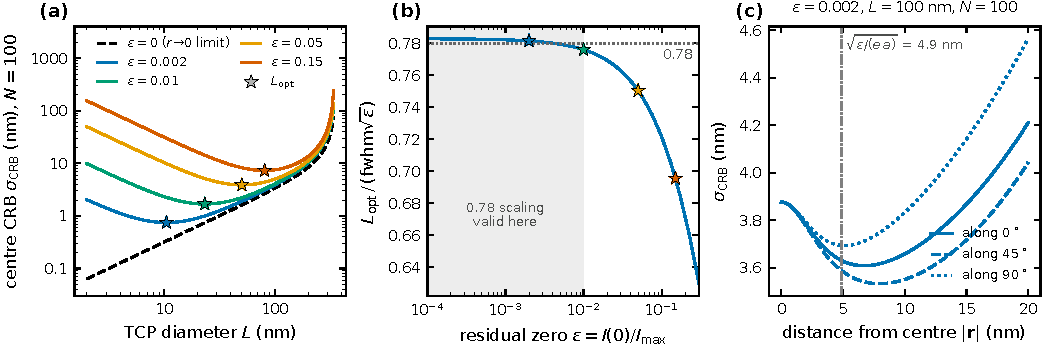
\includegraphics[width=\textwidth]{figures/fig7_zero_depth.pdf}
\caption{Finite zero depth ($\fwhm=\pnum{fwhm_nm}\src{fwhm_nm}$\,nm, $N=100$, Gaussian pedestal).
(a)~Centre CRB versus $L$ for $\epsilon=0.002$, $0.01$, $0.05$, $0.15$ (stars: $L_{\mathrm{opt}}$)
and for $\epsilon=0$ ($r\to0$ limit), which has no optimum and diverges at the ring diameter.
(b)~$L_{\mathrm{opt}}/(\fwhm\sqrt\epsilon)$ versus $\epsilon$: the value
\pnum{L_opt_over_fwhm_sqrt_eps_eps0p002}\src{L_opt_over_fwhm_sqrt_eps_eps0p002} at
$\epsilon=0.002$ holds only for $\epsilon\lesssim0.01$ (shaded) and falls to
\pnum{L_opt_over_fwhm_sqrt_eps_eps0p15}\src{L_opt_over_fwhm_sqrt_eps_eps0p15} at $\epsilon=0.15$.
(c)~CRB (nm) versus distance from the centre along three directions for $\epsilon=0.002$,
$L=100$\,nm: the minimum lies off the centre; the dash-dotted line marks the transition scale
$\sqrt{\epsilon/(ea)}=\pnum{zero_depth_transition_scale_nm}\src{zero_depth_transition_scale_nm}$\,nm,
a scale and not the position of the minimum.}
\label{fig:zerodepth}
\end{figure*}

\begin{figure*}[t]
\centering
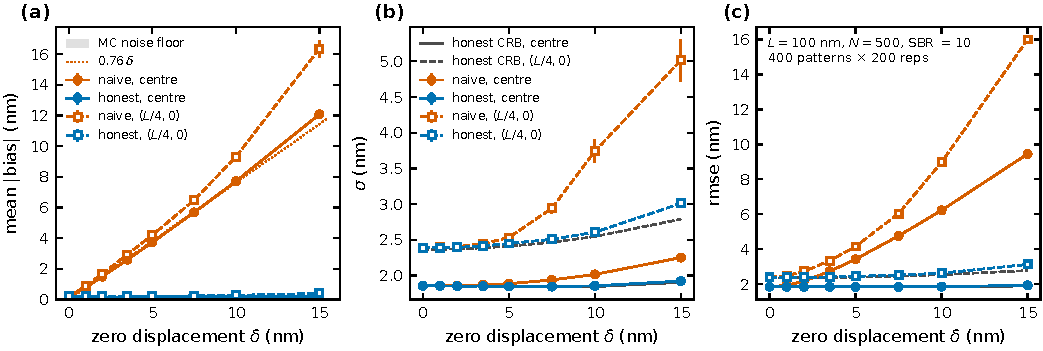
\includegraphics[width=\textwidth]{figures/fig8_misalignment.pdf}
\caption{TCP misalignment, i.e.\ an error in the positions of the zeros with the donut shape
unchanged ($L=100$\,nm, $N=500$, $\sbr=10$; all four zeros displaced by $\delta$
in random directions; $400$ patterns $\times$ $200$ repetitions; error bars are between-pattern
SE). (a)~Mean $|\text{bias}|$ of the naive MLE (nominal pattern) and of the honest MLE (true
pattern) versus $\delta$, at the centre and at $(L/4,0)$, with the MC noise floor (grey band) and
a straight line fitted to the naive centre points over all seven $\delta$ values including
$\delta=15$\,nm (dotted). The main slope estimate is the noise-free population value,
\pnum{misalignment_naive_bias_over_delta_pop_center}\src{misalignment_naive_bias_over_delta_pop_center}
at the centre and
\pnum{misalignment_naive_bias_over_delta_pop_Lq}\src{misalignment_naive_bias_over_delta_pop_Lq}
at $(L/4,0)$, growing with $\delta$. (b)~$\sigma$ and (c)~rmse versus $\delta$, with the CRB of
the true pattern: at the centre the naive $\sigma$ changes little and its loss is bias, whereas
at $(L/4,0)$ the naive $\sigma$ also grows, from
\pnum{misalignment_naive_sigma_Lq_d0_nm}\src{misalignment_naive_sigma_Lq_d0_nm} to
\pnum{misalignment_naive_sigma_Lq_d10_nm}\src{misalignment_naive_sigma_Lq_d10_nm}\,nm at
$\delta=10$\,nm; the honest $\sigma$ follows the CRB at
the centre and lies slightly above it at $(L/4,0)$.}
\label{fig:misalignment}
\end{figure*}

\section{Discussion: what matters experimentally}\label{sec:discussion}

Ordering the effects studied by their numerical impact on the centre precision gives a clear
hierarchy.

\emph{1. The quality of the zero.} A filled zero is the largest effect by far. With the wrong
handedness the centre CRB at $L=50$\,nm rises from
\pnum{crb_center_vec_correct_L50_N100_nm}\src{crb_center_vec_correct_L50_N100_nm}\,nm to
\pnum{crb_center_vec_opposite_L50_N100_nm}\src{crb_center_vec_opposite_L50_N100_nm}\,nm, and
with linear polarization to
\pnum{crb_center_vec_linear_L50_N100_nm}\src{crb_center_vec_linear_L50_N100_nm}\,nm
(Table~\ref{tab:vectorial}). Even a small residual $\epsilon$ matters at small $L$: at $L=50$\,nm
a Gaussian pedestal of $\epsilon=0.05$ multiplies the CRB by
\pnum{crb_eps_degradation_L50_eps0p05_gaussian}\src{crb_eps_degradation_L50_eps0p05_gaussian}
(Table~\ref{tab:eps}). The practical consequence is that $L$ should not be reduced below
$L_{\mathrm{opt}}$ for the measured zero depth (Sec.~\ref{sec:nonideal}); polarization control
of the donut \cite{Lopez2023} comes before any other refinement.

\emph{2. Misalignment with a nominal model.} A displacement $\delta$ of the zeros that is ignored
by the estimator produces a bias of order
\pnum{misalignment_naive_bias_over_delta_pop_center}\src{misalignment_naive_bias_over_delta_pop_center}$\,\delta$
at the centre and larger off-centre. At $\delta=10$\,nm and $N=500$ the bias at the centre
(\pnum{misalignment_naive_bias_abs_center_d10_nm}\,$\pm$\,\pnumse{misalignment_naive_bias_abs_center_d10_nm}\src{misalignment_naive_bias_abs_center_d10_nm}\,nm)
is several times the statistical precision
(\pnum{misalignment_naive_sigma_center_d10_nm}\src{misalignment_naive_sigma_center_d10_nm}\,nm),
and it is invisible in the spread of repeated localizations. Calibrating the actual pattern and
using it in the likelihood removes it (honest MLE).

\emph{3. Background.} At $L=50$\,nm, $N=100$, $\sbr=10$ raises the centre CRB from
\pnum{crb_center_point_S27_L50_N100_nm}\src{crb_center_point_S27_L50_N100_nm}\,nm (point value)
to \pnum{crb_center_sbr10_L50_N100_nm}\src{crb_center_sbr10_L50_N100_nm}\,nm, and the photons
for $5$\,nm from \pnum{photons_for_5nm_L50_sbrinf}\src{photons_for_5nm_L50_sbrinf} to
\pnum{photons_for_5nm_L50_sbr10}\src{photons_for_5nm_L50_sbr10}. Background also regularizes the
model, making the MLE efficient at the centre.

\emph{4. Estimator and protocol.} The MLE is efficient at the centre with background, but not
uniformly inside the pattern at $N=100$
($\sigma/\crb=\pnum{mle_sbr10_sigma_over_crb_x15_N100}\src{mle_sbr10_sigma_over_crb_x15_N100}$
at $15$\,nm from the centre), and the linearized LMS estimators are strongly biased off-centre.
In iterative MINFLUX the search disk and the re-centring are part of the result; a heuristic
$L$ schedule based on the centre CRB leaves a fraction
\pnum{adaptive_frac_outside_next_radius}\src{adaptive_frac_outside_next_radius} of emitters
outside the next pattern.

\emph{5. Definitions.} Without background the centre CRB depends on its definition by the factor
$\rho=\pnum{limit_to_point_ratio_L50}\src{limit_to_point_ratio_L50}$ at $L=50$\,nm; the
background-free MLE even beats both values. Benchmarks against ``the CRB at the centre'' should
state which one is used, or include background.

\emph{6. Beam model.} Once the zero is correct, the scalar LG model is adequate if its size
parameter is chosen to match the curvature of the actual zero: the error in the centre CRB is
then below the percent level (Table~\ref{tab:vectorial}). With the default $\fwhm$ the
discrepancy grows with $L$, reaching a CRB ratio of
\pnum{crb_vec_over_lg300_L150_N100}\src{crb_vec_over_lg300_L150_N100} at $L=150$\,nm.

Iterative MINFLUX reaches a small fraction of the camera precision for the same photons
(\pnum{iterative_ratio_min}\src{iterative_ratio_min}--\pnum{iterative_ratio_max}\src{iterative_ratio_max})
in our idealized setting; the effects above, all absent from that simulation, set how much of
this advantage survives in an experiment.

\section{Limitations and open points}\label{sec:open}

The following points are either not verified or rest on declared choices; they are listed here
rather than stated as results.

\begin{itemize}
\item \emph{Scope of the model.} All simulations are two-dimensional, with a fixed $N$
(multinomial statistics), a background equal in all exposures with the SBR held fixed at every
position (Sec.~\ref{sec:model}), no dipole orientation effects,
no aberrations beyond the zero depth and no drift. The camera reference is ideal
(Sec.~\ref{sec:camera}); real cameras are worse.
\item \emph{rmse normalization.} We use the per-axis convention of Eq.~\eqref{eq:crb} for $\sigma$
and rmse. Whether it coincides with the error definition of Masullo \textit{et al.}
\cite{Masullo2022} was not checked, because the main text of that work is not in our notes.
\item \emph{$\sbr=10$ for the MLE efficiency.} The efficiency at the centre is defined with
$\sbr=10$; this was chosen by the study coordinator on behalf of the author because without
background the model is not regular (Sec.~\ref{sec:estimators}). It is a convention, pending
explicit confirmation by the author.
\item \emph{Vectorial ring diameter versus PyFocus.} Our peak-to-peak diameters of the
vectorial donut as a function of the filling factor ($n=1.5$) agree to within a few percent with
the values we transcribed from Fig.~10 of Ref.~\cite{Caprile2022} at filling factors $0.5$, $2$
and uniform illumination, but differ clearly at filling factor $1$. We do not claim agreement
there; an independent comparison is pending.
\item \emph{Heavy tail at low photon numbers.} In iterative MINFLUX at $N_{\mathrm{tot}}=250$
the error distribution is heavy-tailed and the bootstrap SE of $\sigma$ is itself unstable; the
full-range slope inherits this.
\item \emph{Range dependence of the $L$ exponent.} The exponent
\pnum{crb_exponent_L}\src{crb_exponent_L} applies only to $L\ll\fwhm$; it increases when the fit
range extends to larger $L$.
\item \emph{Three-dimensional donuts and axial misalignment} are outside the scope of this study.
\item \emph{Instrument-level effects} studied with SimuFLUX \cite{MarinRies2026}, i.e.\
misalignment of the vortex phase mask, aberrations, fluorophore blinking and bleaching,
neighbouring emitters, emitter motion, unequal dwell times of the exposures and the validity
filters of commercial instruments, are not modelled here. In particular all our exposures have
the same dwell time.
\end{itemize}

\section{Methods and reproducibility}\label{sec:methods}

\emph{Code.} All computations use our own Python package \texttt{donutloc} (beams, patterns,
photon model, Fisher information, estimators, Monte Carlo, vectorial focusing, iterative
MINFLUX), with NumPy and SciPy only. Each figure has its own script
(\nolinkurl{scripts/fig_*.py}); a single script, \nolinkurl{scripts/compute_paper_numbers.py}, writes
the registry \nolinkurl{data/paper_numbers.json}, from which every number in this paper is typeset
through generated macros; no computed result is typed by hand (only input parameters and
exact constants are). All MC runs use the seed $42$. The central
results have a statistical error below $2\%$; the others are quoted with their SE, namely the
misalignment quantities (where the dispersion between random patterns is intrinsic), the bias
of the background-free MLE at $\rr=(2,0)$\,nm\src{mle_nobg_bias_x_r2_nm} and the fraction of
emitters left outside the next pattern by the adaptive $L$ schedule\src{adaptive_frac_outside_next_radius}. The closed forms of
App.~\ref{app:derivation} are checked against a numerical Fisher computation by
\nolinkurl{scripts/verify_crb_closed_forms.py} and by unit tests. A reproduction script in
\nolinkurl{scripts/} runs, in order, the tests, the figures, the number registry and the provenance
check.

\emph{Provenance.} Every quantitative statement carries a tag that resolves in
\nolinkurl{paper/provenance.json} to the script, check or derivation that reproduces it;
\nolinkurl{scripts/check_provenance.py} verifies that every tag and every number resolves and that
the generated macros are in sync with the registry.

\emph{How the study was made.} The study was carried out with an agent team following the
agent-team methodology \cite{agentteam}: bounded rounds in which worker agents derive and
compute, an independent verifier re-derives or recomputes every claim by a separate route before
it is accepted, and a writer transcribes only verified claims with provenance-checked numbers.
The complete audit trail (ledger of claims with their status, per-round reports and human
decisions) is kept in \nolinkurl{equipo/2026-09-26_donut-localization/} of the repository. The
author set the questions, the conventions and the acceptance test.

\begin{acknowledgments}
The simulations, derivations and the draft of this manuscript were produced with a team of AI
agents under the agent-team methodology \cite{agentteam}, with independent verification of every
reported claim; the author directed the study and is responsible for its content.
\end{acknowledgments}


\appendix
\section{Closed forms for the CRB at the TCP centre}\label{app:derivation}

This appendix transcribes the derivation in \nolinkurl{docs/derivations/crb_tcp_center.md}\src{deriv_master_formula}; every boxed result there is implemented in
\nolinkurl{src/donutloc/closed_forms.py} and checked against a numerical Fisher matrix\src{check_closed_forms}. Equation numbers S$n$ refer to the Supplementary Material of
Ref.~\cite{Balzarotti2017}.

\subsection{Notation}
Write every exposure as $\lambda_i(\rr)=h(|\rr-\bb_i|^2)$ with $\bb_i$ from Eq.~\eqref{eq:tcp},
$R=L/2$, and for the LG donut $h(u)=e\,a\,u\,e^{-au}$. Define $x\equiv aR^2=L^2\ln2/\fwhm^2$ and
$g\equiv1-x$. Since $\sum_ke^{i\varphi_k}=\sum_ke^{2i\varphi_k}=0$,
\begin{equation}
\sum_{k=0}^{2}\bb_k=\mathbf0,\qquad\sum_{k=0}^{2}\bb_k\bb_k^{T}=\tfrac32R^2\,\mathbb{I} .
\label{eq:triangle}
\end{equation}

\subsection{Master formula}
With $h_R\equiv h(R^2)$, $h'_R\equiv h'(R^2)$ and $h_0\equiv h(0)$,
$\lambda_k=h_R-2h'_R\,\bb_k\cdot\rr+O(r^2)$ for the peripheral exposures and
$\lambda_3=h_0+h'(0)r^2+O(r^4)$. By Eq.~\eqref{eq:triangle} the linear term of
$S=\sum_j\lambda_j$ cancels, $S=S_0+O(r^2)$ with $S_0=3h_R+h_0$. At $\rr=\mathbf0$,
$\nabla p_k=-2h'_R\bb_k/S_0$ and $\nabla p_3=\mathbf0$, and the three peripheral terms of
Eq.~\eqref{eq:fisher} give
\begin{equation}
F=\frac{6NR^2\,h_R'^2}{h_R\,(3h_R+h_0)}\;\mathbb{I} ,
\label{eq:master}
\end{equation}
valid for any radial beam provided the central term vanishes at the origin. A background $b$
per exposure amounts to $h_R\to h_R+b$ and $3h_R+h_0\to S_0+4b$.

\subsection{Point value}
For the LG donut $h_R=exe^{-x}$, $R^2h'_R=ex(1-x)e^{-x}$ and $h_0=0$. Equation~\eqref{eq:master}
gives $F=(8Ng^2/L^2)\,\mathbb{I}$, hence Eq.~\eqref{eq:s27} (Eq.~S27), with the central $0/0$ term
excluded.

\subsection{Limit $r\to0$}
For $\rr\neq\mathbf0$, $p_3=ea\,r^2/S_0\,[1+O(r^2)]$ and $\nabla p_3=2ea\,\rr/S_0\,[1+O(r^2)]$, so
the central term is\src{deriv_limit}
\begin{equation}
\frac{\nabla p_3\nabla p_3^{T}}{p_3}=\frac{4ea}{S_0}\,\rhat\rhat^{T}+O(r^2)
=\frac{16\,e^{x}}{3L^2}\,\rhat\rhat^{T}+O(r^2).
\end{equation}
The $O(r)$ changes of the peripheral terms are odd in $\rhat$ and do not contribute to the limit
of the trace. Therefore
\begin{equation}
F_{\lim}(\rhat)=\alpha\,\mathbb{I}+\beta\,\rhat\rhat^{T},\qquad
\alpha=\frac{8Ng^2}{L^2},\qquad\beta=\frac{16Ne^{x}}{3L^2},
\label{eq:alphabeta}
\end{equation}
with eigenvalues $\alpha+\beta$ (along $\rhat$) and $\alpha$ (across). The trace
$\mathrm{tr}F_{\lim}^{-1}=1/\alpha+1/(\alpha+\beta)$ does not depend on $\rhat$, and
Eq.~\eqref{eq:crb} gives Eq.~\eqref{eq:limit}. For $x\to0$, $\beta/\alpha=2/3$ and
$\rho^2=4/5$, i.e.\ $\rho=2/\sqrt5$ and $\sigma_{\lim}^2=L^2/(10N)$; for small $x$,
$\rho\simeq(2/\sqrt5)(1-9x/40)$. The axes of the limiting error ellipse are
$\sigma_\parallel=(\alpha+\beta)^{-1/2}$ and $\sigma_\perp=\alpha^{-1/2}=\sigma_{\mathrm{pt}}$,
with ratio $\sqrt{3g^2/(3g^2+2e^{x})}$, equal to $\sqrt{3/5}$ for a quadratic zero.

The discontinuity\src{deriv_discontinuity}: the central term has norm $\beta/N$ but direction
$\rhat$, so it has no matrix limit at $\mathbf0$ (its trace does); assigning it the value zero
(the S27 convention) matches no directional limit. Equivalently, with
$F=4N\sum_i\nabla\sqrt{p_i}\,\nabla\sqrt{p_i}^{T}$, $\sqrt{p_3}\simeq\sqrt{ea/S_0}\,|\rr|$ is a
cone, not differentiable at the origin.

\subsection{Background}
Eq.~S30 with $s=\sbr/(\sbr+1)$ is identical to adding $b=S/(4\,\sbr)$ to each $\lambda_i$. With
$h_0=0$, $h_R+b=h_R(1+\tfrac{3}{4\sbr})$ and $S_0+4b=S_0(1+\tfrac{1}{\sbr})$; Eq.~\eqref{eq:master}
gives Eq.~\eqref{eq:s31} (Eq.~S31). Now $p_3\ge(1-s)/4>0$ and $\nabla p_3=O(r)$, so the central
term vanishes as $r^2$: the CRB is continuous. Near the origin
$\lambda_3+b\simeq ea\,r^2+b$ and the central term is
$[4ea/(S_0+4b)]\,[r^2/(r^2+r_c^2)]\,\rhat\rhat^{T}$ with
$r_c=(\sqrt3L/4)\,e^{-x/2}/\sqrt{\sbr}$ (leading order, $r_c\ll L$). Hence the non-commuting
limits of Sec.~\ref{sec:crb}\src{deriv_noncommuting}.

\subsection{Finite zero depth}
\emph{Constant pedestal}, $h=h_{\mathrm{LG}}+\epsilon$: it is exactly a background $b=\epsilon$
for all $\rr$, so at the centre\src{deriv_pedestal}
\begin{equation}
\begin{gathered}
\crb(\mathbf0)=\sigma_{\mathrm{pt}}\sqrt{\Big(1+\frac{1}{\sbr_\epsilon}\Big)\Big(1+\frac{3}{4\,\sbr_\epsilon}\Big)},\\
\sbr_\epsilon=\frac{3e\,x\,e^{-x}}{4\epsilon}.
\end{gathered}
\end{equation}
With an additional background of given SBR measured against the full beam, pedestal included,
$1+1/\sbr_{\mathrm{eff}}=(1+1/\sbr)(1+1/\sbr_\epsilon)$ and the CRB is Eq.~\eqref{eq:s31} at
$\sbr_{\mathrm{eff}}$.

\emph{Gaussian pedestal}, $h=(ea\,u+\epsilon)e^{-au}$: $h_R=(ex+\epsilon)e^{-x}$,
$R^2h'_R=(exg-\epsilon x)e^{-x}$ and $h_0=\epsilon$, so that
\begin{equation}
\frac{F_\epsilon}{F_{\mathrm{pt}}}=\frac{3x^2(eg-\epsilon)^2}{g^2\,D_\epsilon},\qquad
D_\epsilon=(ex+\epsilon)\,[3(ex+\epsilon)+\epsilon e^{x}],
\end{equation}
with $\crb=\sigma_{\mathrm{pt}}\sqrt{F_{\mathrm{pt}}/F_\epsilon}$.
It is not equivalent to a background: the pedestal is $\epsilon$ at the central exposure and
$\epsilon e^{-x}$ at the peripheral ones, and it reduces the slope by the factor
$1-\epsilon/(eg)$. To first order in $\epsilon$ the two models differ by a relative factor
$1+\tfrac37x^2+O(x^3)$ in the coefficient of $\epsilon$. In both models $p_3(\mathbf0)>0$, the
CRB is continuous at the origin, and it tends to $\sigma_{\mathrm{pt}}$ as $\epsilon\to0$. The
transition radius $\sqrt{\epsilon/(ea)}$ is independent of $L$.

\subsection{Multiphoton exponent}
For $\lambda\propto I^c$, $h(u)=(ue^{-au})^c$, $h'_R/h_R=cg/R^2$ and $h_0=0$, so
Eq.~\eqref{eq:master} gives $F=2Nc^2g^2/R^2$ and
$\sigma_{\mathrm{pt}}^{(c)}=L\,g^{-1}/(2c\sqrt{2N})$\src{deriv_multiphoton}. The central term
scales as $r^{2c-2}$ and vanishes at the origin for $c>1$, so the limit equals the point value.


\bibliography{references}

\end{document}
